\documentclass[12pt,twoside]{scrartcl}
\usepackage[ngerman]{babel} 
\raggedbottom


\usepackage[T1]{fontenc}
\usepackage{lmodern}
\usepackage{graphicx}
\usepackage{amsmath,amssymb,amsfonts,amsthm}
%\usepackage{xfrac} 
\usepackage{bm}
\usepackage[onehalfspacing]{setspace} %das macht die große Lücke
\usepackage{tocbibind}
\usepackage{bibgerm}
\usepackage{wrapfig}
\usepackage{subfigure} 																	
\usepackage{enumitem} 
\usepackage{lastpage} %Z?hlt die Gesamtseitenzahl. Mit \pageref{LastPage} wird diese ausgegeben
\usepackage{hyperref}
\usepackage{bookmark}
\hypersetup{linktoc=all, colorlinks=true, linkcolor=black, urlcolor=black, citecolor=black}
\usepackage{mdframed}
\usepackage{lipsum}
\usepackage{float}
\usepackage{scrextend} 
\usepackage{geometry} 
\usepackage{url}
\usepackage{diagbox}

\usepackage[]{algorithm2e}
\SetArgSty{}
\geometry{a4paper, top=35mm, left=25mm, right=25mm, bottom=25mm, headsep=10mm, footskip=10mm} %Headsep beschreibt 
\usepackage{fancyhdr}
\pagestyle{fancy}
\fancyhead{}
\fancyhead[LE]{\textit{\nouppercase{\leftmark}}}
\fancyhead[RO]{\textit{Das Buffonsche Nadelproblem und die Multi-Level-Monte-Carlo-Methode}}
%\fancyhead[LO,RE]{\thepage}
%\fancyfoot{\thepage}
\fancyfoot[C]{\thepage}
\addtolength{\headheight}{0.15cm}
\usepackage[usenames,dvipsnames,svgnames,table]{xcolor}
\usepackage{tikz}
\usepackage{sectsty}
\definecolor{Mittelblau}{RGB}{0,81,158}
\setlength{\parindent}{0em} 


\newtheoremstyle{satz}% name
{15pt}% Space above
{5pt}% Space below
{\itshape}% Body font
{}% Indent amount: Indent amount: empty = no indent, \parindent = normal paragraph indent
{\bfseries}% Theorem head font
{:}% Punctuation after theorem head
{\newline}% Space after theorem head: Space after theorem head: { } = normal interword space; \newline = linebreak
{}% Theorem head spec (can be left empty, meaning `normal')

\newtheoremstyle{bsp}% name
{15pt}% Space above
{5pt}% Space below
{}% Body font
{}% Indent amount: Indent amount: empty = no indent, \parindent = normal paragraph indent
{\bfseries}% Theorem head font
{:}% Punctuation after theorem head
{\newline}% Space after theorem head: Space after theorem head: { } = normal interword space; \newline = linebreak
{}% Theorem head spec (can be left empty, meaning `normal')


\newcommand{\td}[1]{\text{ d} #1}
\newcommand{\thistheoremname}{}
\theoremstyle{satz}
%Satz
\newtheorem{sz}{Satz}[section]


%Lemma
\newtheorem{vor}[sz]{Voraussetzung}
\newtheorem{alg}[sz]{Algorithmus}
\newtheorem{lem}[sz]{Lemma}
\newtheorem{kor}[sz]{Korollar}
\newtheorem{prop}[sz]{Proposition}
\newtheorem{gsz}[sz]{\thistheoremname}
\newtheorem*{gthm_no_num}{\thistheoremname}
\newtheorem{gd}[sz]{\thistheoremname}

\newtheorem*{gdf_no_num}{\thistheoremname}

%Bsp
\theoremstyle{bsp}
\newtheorem{bsp}{Beispiel}[section]
\newtheorem{df}[sz]{Definition}


\begin{document}

% Titelseite soll keine Kopf oder Fußzeile haben
\thispagestyle{empty}

% Alle Elemente sollen zentriert sein
\begin{center}


\hspace{-2cm}

\includegraphics[width=0.6\textwidth]{_unilogo.png}
\vspace{-0.6 cm}

\hspace{2,2cm}
\\[1cm]
{\Large Institut f"ur angewandte Analysis und Numerische Simulation (IANS)}


\vspace*{3cm}

% Art der Arbeit => (Bachelorarbeit ,Diplomarbeit, Masterarbeit, Seminararbeit)
\Large{\textbf{Masterarbeit}\\

\vspace{2cm}

% Titel der Arbeit 
\textbf{{\Large{Optimierung der Multi-Level-Monte-Carlo-Methode f"ur das Buffonsche Nadelproblem}}}

\vspace*{1mm}


\vspace{4cm}


% Gutachter, Kontaktdaten und Abgabetermin
\parbox{120mm}{
\begin{large}
\begin{tabbing}
Betreuerin: \hspace{0.7cm} \= Prof. Andrea Barth\\[4mm]
Verfasser:\> Mystery Math Girl\\ % alphabetische Reihenfolge (Nachname)
Matrikel-Nr.:\> 9999999\\
Email:\>mystery.math.girl@unknown.de\\
%\textbf{Abgabetermin:} \hspace{0,3cm} \> \textbf{01. Januar 2017}\\
\end{tabbing}
\end{large}
 }}
\end{center}

 
%deckblatt ende
\newpage 
\thispagestyle{empty}
\quad  
\newpage
\thispagestyle{empty}
\begin{center}
\textbf{\Large{Danksagung}}\\[2cm]
\begin{flushleft}
Zuerst m"ochte ich mich bei Prof. Andrea Barth f"ur die ausgezeichnete Betreuung dieser Arbeit bedanken. \\
Dank geb"uhrt au"serdem meinem Kommilitonen Philipp Beck f"ur das Korrekturlesen meiner Arbeit und die vielen Diskussionen "uber mein Thema.
Ein gro"ser Dank geht an meine Eltern, meine Schwester und wiederum Philipp Beck, die mich w"ahrend meines gesamten Studiums unterst"utzt und auch in schwierigeren Situationen stets motiviert und ermutigt haben.
\end{flushleft}
\end{center}\vspace{2cm}
%\newpage
\newpage 
\thispagestyle{empty}
\quad  
\newpage
\fancyfoot[C]{}
\tableofcontents
\newpage
\thispagestyle{empty}
\fancyfoot[C]{\thepage}

\quad  
\newpage
\section{Einleitung}
Die Monte-Carlo-Simulation oder Monte-Carlo-Studie, auch MC-Simulation genannt, ist ein Verfahren aus der Stochastik, bei dem eine sehr gro"se Zahl gleichartiger Zufallsexperimente die Basis darstellt. Es wird dabei versucht, analytisch nicht oder nur aufwendig l"osbare Probleme mit Hilfe der Wahrscheinlichkeitstheorie numerisch zu l"osen. Als Grundlage ist vor allem das Gesetz der gro"sen Zahlen zu sehen.
Anwendung findet die Monte-Carlo-Methode in vielen Bereichen. Neben der numerischen Mathematik werden die Monte-Carlo-Methoden auch in der Physik, Finanzwirtschaft und in den Ingenieurwissenschaften verwendet.\\
Das gr"o"ste Problem an dieser Methode liegt darin, dass ein hoher Grad an numerischer Genauigkeit auch einen hohen numerischen Aufwand mit sich bringt. Dies erfordert also eine Abw"agung zwischen hoher Pr"azision auf der einen Seite und einem m"oglichst niedrigen Rechenaufwand auf der anderen Seite. Damit stellt sich die Frage wie sich der Rechenaufwand des Verfahrens verringern l"asst, jedoch die Genauigkeit nicht darunter leidet. Eine Antwort bietet das Multi-Level-Monte-Carlo-Verfahren, bei dem durch die Variation der Diskretisierungsschrittweiten bei der Simulation eine Verringerung der Anzahl an notwendigen Simulationen erzielt werden kann.\\[0,1cm]
Diese Arbeit befasst sich mit dem  Buffonschen Nadelproblem und der Anwendung und Optimierung von Monte-Carlo-Algorithmen darauf. 
Das Buffonsche Nadelproblem besch"aftigt sich mit der Wahrscheinlichkeit, mit welcher  eine willk"urlich geworfene Nadel ein Gitter paralleler Linien schneidet. Es erlaubt unter anderem, die Kreiszahl 
$\pi$  experimentell zu bestimmen. Das Problem geh"ort zum Bereich der Integralgeometrie und war eines der ersten auf diesem Gebiet. Georges-Louis Leclerc de Buffon behandelte es erstmals 1733 vor der Pariser Akademie der Wissenschaften. 
Georges-Louis Leclerc, Comte de Buffon (geb. am September 1707 in Montbard; gestorb. 16. April 1788 in Paris) war ein franz"osischer Naturforscher im Zeitalter der Aufkl"arung.\\

Wir werden zuerst die klassische Monte-Carlo-Methode auf dieses Problem anwenden und dann zur Multi-Level-Monte-Carlo-Methode "ubergehen.
Anschlie"send ist das Ziel diese Methoden f"ur das Problem zu optimieren.\\
Als Erstes ist unser Ziel, bei einer gegebenen Levelanzahl und Fehlertoleranz die optimale Anzahl an Samples pro Level zu bestimmen.
Dabei bestimmen wir die L"osung eines allgemeineren Optimierungproblemes und zeigen, dass diese bei uns anwendbar ist.
Danach besch"aftigen wir uns mit dem Problem, wie die Levelanzahl und Sampleanzahl bei gegebener Rechenkapazit"at zu w"ahlen ist, um den Fehler minimal zu halten. Dabei werde ich zwei unterschiedliche Vorgehensweisen vorstellen.\\ Bei beiden Methoden werde ich zuerst die optimale Sampleverteilung bei gegebenen Kostenbudget und gegebener Levelanzahl bestimmen. Erst danach betrachte ich das Problem, welche Anzahl an Leveln den minimalen Fehler liefert.\\
Die erste Vorgehensweise ist die Lagrange-Multiplikator-Methode. Da wir ein Optimierungsproblem mit Nebenbedingung vorliegen haben, ist dies eine geeignete M"oglichkeit. Unser Optimierungsproblem ist aber diskret, was wir nat"urlich noch ber"ucksichtigen m"ussen.
Bei der zweiten Vorgehensweise versuche ich das Problem direkt diskret mit einer angepassten Form des Greedy-Algorithmus zu l"osen. Abschlie"send werde ich die Ergebnisse der beiden Methoden  sowie die Ergebnisse der zwei unterschiedlichen Optimierungsprobleme vergleichen.\\[0,2cm]





\newpage
\subsection{Einf"uhrung in die Monte-Carlo-Methode}

Monte-Carlo-Methoden sind Algorithmen, die Zufallszahlen nutzen um nicht oder nur aufwendig l"osbare Probleme stochastisch zu approximieren. Wie in der Einleitung schon genannt, liefert die Grundlage hierf"ur das starke Gesetz der gro"sen Zahlen.
In diesem Kapitel orientiere ich mich an \cite{MC}.
\begin{sz}[Starkes Gesetz der gro"sen Zahlen]
Sei $(X_i, i\in\mathbb{N})$ eine Folge unabh"angiger, identisch verteilter
Zufallsvariablen in $L^1$. Dann konvergiert die Folge $(S_n, n \in \mathbb{N})$
mit $S_n := \frac{1}{n}\sum_{i=1}^n X_i$ 
fast sicher gegen $\mathbb{E}(X_1).$
\end{sz}
Allgemeines Ziel ist die Approximation einer reellen Zahl $a$. Man konstruiert dann eine reellwertige Zufallsvariable $Y$ mit 
$\mathbb{E}(Y) = a.$\\
$Y$ hei"st \textbf{Basisexperiment} der direkten Simulation.
Man betrachtet anschlie"send eine Folge $(Y_i)_{i\in\mathbb{N}}$ von reellwertigen, unabh"angigen
Zufallsvariablen mit gleicher Verteilung wie Y.
Diese nennt man auch unabh"angige \textbf{Kopien} oder
\textbf{Wiederholungen} von Y.
Die Zahl $a$ wird nun durch $D_n =\frac{1}{n}\sum_{i=1}^n Y_i$ approximiert.
$D_n$ hei"st direkte Simulation oder \textbf{Monte-Carlo-Sch"atzer}.
\begin{sz}\label{var}
F"ur den Fehler der direkten Simulation gilt:
\begin{align*}
\Delta (D_n)=\sqrt{\mathbb{E}(D_n-a)^2}=\sqrt{\frac{Var(Y)}{n}}.
\end{align*}
\end{sz}
\begin{proof}
Es ist 
\begin{align*}
\mathbb{E}(D_n-a)^2= Var(D_n)=Var\left(\frac{1}{n}\sum_{i=^1}^n Y_i\right)=\frac{1}{n^2}Var\left(\sum_{i=^1}^n Y_i\right)\underset{(*)}{=}\frac{1}{n^2}\cdot n\cdot Var(Y)=\frac{Var(Y)}{n}
\end{align*}
$(*)$ da  $Y_i$ unabh"angig 
\end{proof}

\begin{df}[Landau-Symbol]
Gegeben seien zwei reellwertige Funktionen $g,h$. Dann hei"st $g(x)$ von der Ordnung $h(x)$, also $g(x)=\mathcal{O}(h(x))$ falls gilt:
\begin{align*}
\exists C>0 \ \ \exists x_0>0\ \ \forall x>x_0\ : \ |g(x)|\leq C \cdot |h(x)|.
\end{align*}
\end{df}

Mit dieser Definition und obigem Satz gilt also: $Var(D_n)=\mathcal{O}(\frac{1}{n}).$\newpage
\begin{enumerate}
\item \textbf{Die Hit-or-Miss Integration}:\\
Das Ziel ist es eine Funktion $f:[0,1]\rightarrow \mathbb{R}$ zu integrieren.
Bei der Hit-or-Miss Integration macht man direkten Gebrauch von der Interpretation des Integrals als Fl"acheninhalt A.
Wir haben einen Wahrscheinlichkeitsraum $(\Omega,\mathcal{A},\mathbb{P})$ und betrachten die Zufallsvariable $Y=\mathbb{I}_A$.
Die zu untersuchende Fl"ache A wird durch ein Rechteck eingegrenzt und
auf diesem werden mit einer Gleichverteilung zuf"allige Punkte
erzeugt.\\
Es gilt dann $\mathbb{E}(Y ) = \mathbb{P}(A) =\frac{ \text{gesuchter Fl"acheninhalt}}{\text{Fl"ache Rechteck}}$.
Dank dem SGdgZ konvergiert $\frac{\text{Anzahl Treffer}}{\text{Anzahl der Punkte}}$ gegen die Wahrscheinlichkeit $\mathbb{E}(Y)=\mathbb{P}(A)$.
\item \textbf{Direkte Monte-Carlo Integration}:\\
Wiederum ist das Ziel das Integral einer Funktion $f:D\rightarrow \mathbb{R}$ zu approximieren.
Jetzt werden aber aber im Definitionsbereich zuf"allige Werte erzeugt und $f$ wird an diesen Stellen ausgewertet und der Mittelwert dieser Funktionswerte gebildet.
D.h das Integral $S(f) = \int_D f(x) \ \text{dx}$ wird approximiert durch $ M(f) =\frac{1}{n}\sum_{i=1}^n f(X_i)$
mit einer Folge von auf $D$ gleichverteilten,unabh"angigen
Zufallsvektoren $X_i$.
\end{enumerate}

\subsubsection{Beispiel: Berechnung von $\pi$}
In diesem Beispiel wollen wir $\pi$ mit Hilfe des Einheitskreises bzw. eines Einheitskreisviertels berechnen.
Genauer betrachten wir die Menge $G=[0,1]^2$.
\begin{enumerate}
\item[a)]\underline{Die Hit-or-Miss-Methode:}\\
Das Basisexperiment ist die Zufallsvariable $Y := \mathbb{I}_B $ mit \\ 
$B=\{(x_1, x_2) \in G | \  x_1^2+x_2^2\leq1\}$.
Es gilt dann $\mathbb{P}(B) =\mathbb{E}(Y ) =\frac{\pi}{4}$.\\
W"ahlt man nun also zuf"allige Punkte im Einheitsquadrat und bestimmt
den relativen Anteil der Punkte in B, bekommt man eine Approximation
von $\frac{\pi}{4}$. Das bedeutet $4\cdot \frac{\text{Punkte in B}}{\text{Punkte gesamt}}\approx \pi$.
\begin{figure} [H]
\centering
    \subfigure[$n=10^2$]{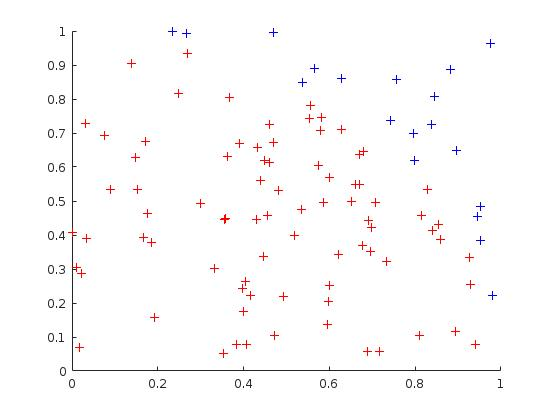
\includegraphics[width=5cm]{10^2.jpg}} 
    \subfigure[$n=10^3$]{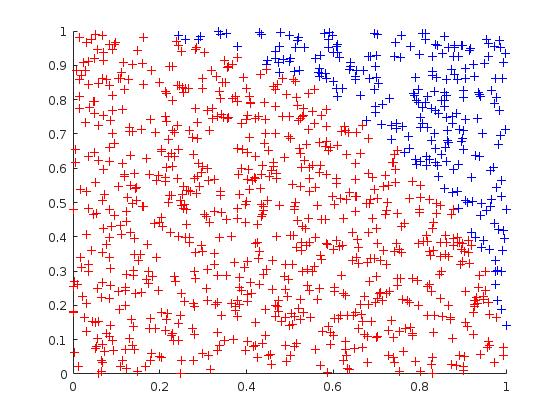
\includegraphics[width=5cm]{10^3.jpg}} 
    \subfigure[$n=10^5$]{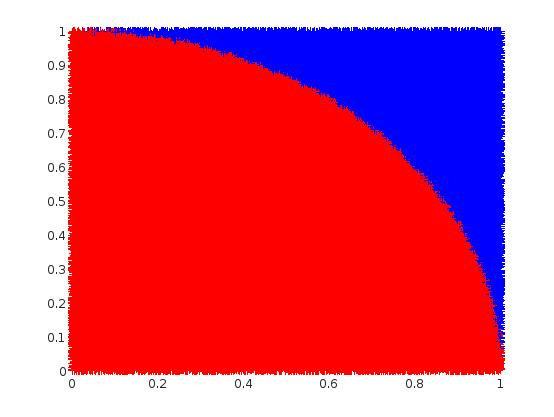
\includegraphics[width=5cm]{10^5.jpg}} 
\end{figure}
\newpage
Die Ergebnisse waren f"ur mehrere Durchl"aufe:
\begin{enumerate}
\item[-]$n=10^2$: $3,24; 3,28; 2,96$
\item[-]$n=10^3$: $3,125; 3,128; 3,104$
\item[-]$n=10^5$: $3,1415; 3,1472; 3,1371$.
\end{enumerate}
\item[b)]\underline{Direkte Simulation:}\\
Wir betrachten die Funktion $g(x)=\sqrt{1-x^2}$. Es seien au"serdem $X_i$ auf $[0,1]$  gleichverteilte unabh"angige Zufallsvariablen. Der Monte-Carlo-Sch"atzer ist dann gegeben durch $D_n:=\frac{1}{n}\sum_{i=1}^n g(X_i)$.

\begin{figure}[H]
\centering
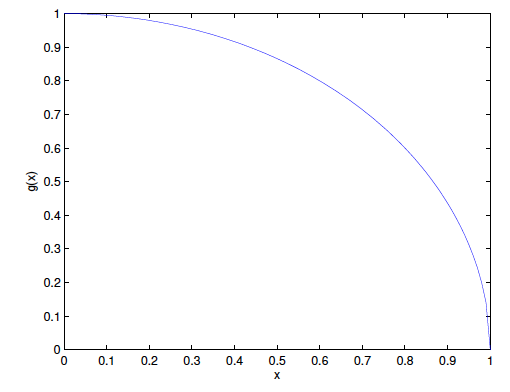
\includegraphics[width=9cm]{Kreis.jpg}
\caption{ Graph der Funktion $g(x)$}
\end{figure}
\begin{figure}[H]
\centering
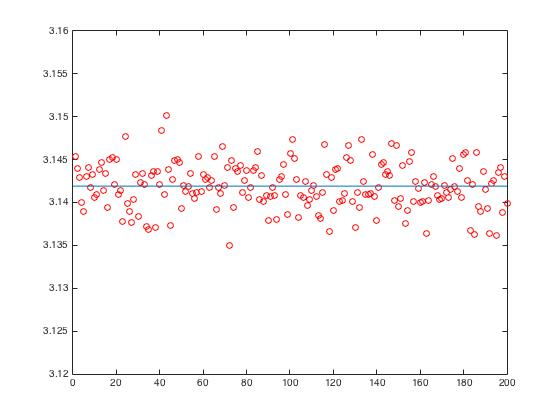
\includegraphics[width=9cm]{direkt200.jpg}
\caption{ Ergebnisse von 200 Durchl"aufen}
\end{figure}

\end{enumerate}
\newpage 
\thispagestyle{empty}
\quad  
\newpage
\section{Das Buffonsche Nadelproblem}

In diesem Kapitel werden wir nun das Buffonsche Nadelproblem genauer betrachten. Im Jahre 1733 stellte sich Buffon folgende Frage:\\
\textit{Mit welcher Wahrscheinlichkeit schneidet eine willk"urlich geworfene Nadel ein Gitter paralleler Linien?}\\

\underline{\textbf{Probleml"osung bzw. experimentelle Durchf"uhrung:}}\\[0,2cm]

Ben"otigt werden m"oglichst viele identische Nadeln gleicher L"ange $l$. Auf einer Ebene werden parallele Linien mit einem bestimmen Abstand $d$ konstruiert. Die Nadeln werden anschlie"send auf diese Ebene geworfen und es wird gez"ahlt, wie viele dieser geworfenen Nadeln eine Linie kreuzen.\\ Man stellt fest, dass man dadurch eine Ann"aherung der Zahl $\pi$ bekommt.\\
Wir betrachten in unserem Problem Nadeln der L"ange $\lambda \in [0,1]$, die nacheinander auf eine Ebene mit Linien mit Abstand $1$ geworfen werden.  Um eine Antwort auf obige Frage zu erhalten, f"uhren wir folgende Menge  $\Omega=[0,\frac{1}{2}]\times [0,\frac{\pi}{2}] $ ein.\\
Dabei repr"asentiert bei $(x,\alpha)\in \Omega$ die erste Komponente $x$ den Abstand vom Mittelpunkt der Nadel zur n"achsten parallelen Linie in der Ebene. Die zweite Komponente $\alpha$ beschreibt den Winkel, der von der Nadel und der getroffenen Linie eingeschlossen wird.

\begin{figure} [H]
\centering
    \subfigure[Nadeln auf Ebene]{
		\begin{tikzpicture}
		\draw (0,0) -- (6,0);
		\draw (0,1) -- (6,1);
		\draw (0,2) -- (6,2);
		\draw (0,3) -- (6,3);
		\draw (0,4) -- (6,4);

\draw [blue](0.5,2.8) -- +(20:1cm);
\draw [blue](2.6,3.4) -- +(-30:1cm);
\draw [blue](5.5,3.1) -- +(215:1cm);

\draw [blue](1.3,2.4) -- +(260:1cm);
\draw [blue](2.6,2.3) -- +(310:1cm);
\draw [blue](4.5,1.6) -- +(55:1cm);

\draw [blue](1.6,1.4) -- +(-35:1cm);
\draw [blue](3.7,1.3) -- +(-85:1cm);

\draw [blue](1.1,0.1) -- +(5:1cm); 
\draw [blue](5.3,0.3) -- +(60:1cm);
		\end{tikzpicture}    
    
    } 
    \subfigure[Genaue Betrachtung einer Nadel der L"ange 1]{
    \begin{tikzpicture}[scale =3.5]

\definecolor{dunkelg}{RGB}{0,119,30};

\draw[very thin] (0,0)   -- (2,0);
\draw[very thin] (0,0.5) -- (2,0.5);
\draw[very thin] (0,1)   -- (2,1);

\draw[very thin] (1,0) -- (1,1);

\draw[<->,ultra thin] (-0.07,0) -- (-0.07,1);
\draw[<->,ultra thin] (2.07,0) -- (2.07,0.5);

\draw[very thin] (1.5,0)  arc[radius = 5mm, start angle= 0, end angle= 90];

\draw[very thin,blue] (1.6,0.35) -- +(210:1cm);

\draw[very thin,dunkelg] (1.4,0)  arc[radius = 4mm, start angle= 0, end angle= 30];

\draw[fill,blue] (0.748,-0.145) circle [radius = 0.01];
\draw[fill,blue] (1.6,0.35) circle [radius = 0.01];
\draw[fill,blue] (1.15,0.09) circle [radius = 0.01];


\draw[ultra thin] (0.97,0.253) -- (1.43,0.253);

\node[scale =0.9] at (2.15,0.25) {$\frac{1}{2}$};
\node[scale =0.9] at (-0.15,0.5) {$1$};
\node[scale =0.9] at (0.9,0.09) {$x$};
\node[scale =0.8] at (0.80,0.253) {	$\frac{1}{2} \sin(\alpha)$};

\node[dunkelg,scale=0.9] at (1.24,0.06) {$\alpha$};
\draw[ultra thin] (0.97,0.09) -- (1.15,0.09);

\draw[fill,blue] (1.15,0.09) circle [radius = 0.01];
\end{tikzpicture}
    
    
    } 
\caption{Modellierung des Nadelproblems} 
\end{figure} 
Um den zuf"alligen Wurf zu modellieren betrachten wir den Wahrscheinlichkeitsraum $(\Omega,\mathcal{F},\mathbb{P})$  und versehen $\Omega$ mit der Borel-$\sigma$-Algebra.\\ D.h es ist $\mathcal{F}=\mathcal{B}\left([0,\frac{1}{2}]\times[0,\frac{\pi}{2}]\right)$ und wir haben das Wahrscheinlichkeitsma"s\\ $\mathbb{P}=(2 \ dx) \otimes(\frac{2}{\pi} \ d\alpha)$.\\
Die Menge 
\begin{align*}
B_\lambda=\left\{(x,\alpha)\in \Omega: x\in [0,\frac{\lambda}{2}\sin(\alpha)]\right\}
\end{align*}
beschreibt dann das Ereignis, dass eine Linie getroffen wird.\\
Dann ist f"ur jedes $\lambda\in[0,1]$ die exakte L"osung bzw. die Antwort zu unserem Problem gegeben durch 
\begin{align*}
\mathbb{P}(B_\lambda)&=\frac{2}{\pi}\int_0^\frac{\pi}{2} 2 \int_0^\frac{1}{2} \mathbb{I}_{[0,\frac{\lambda}{2}\sin(\alpha)]}(x)\text{d}x \text{d}\alpha\\&=\frac{4}{\pi}\int_0^\frac{\pi}{2}\frac{\lambda}{2}\sin(\alpha)\text{d}\alpha=\frac{2\lambda}{\pi}:=a(\lambda).
\end{align*}
Unser Ziel ist es die klassische Monte-Carlo-Methode sowie die Multi-Level-Monte-Carlo-Methode anzuwenden um die exakte L"osung $[0,1]\ni \lambda \longmapsto a(\lambda)\in [0,1]$ f"ur alle $\lambda \in [0,1]$ zu approximieren.
Daf"ur nehmen wir an, dass gilt $a\in H=L^2([0,1]).$ D.h. $a$ ist ein Element des Hilbertraumes der quadratisch integrierbaren Funktionen versehen mit dem Standardskalarprodukt
\begin{align*}
\langle f,g \rangle=\int_0^1 f(x)g(x) \text{d}x.
\end{align*}
Au"serdem betrachten wir die folgende Indikatorfunktion
\begin{align*}
f:\Omega\times[0,1]\rightarrow \{0,1\} \ \text{mit} \ f(x,\alpha,\lambda)=\mathbb{I}_{B_\lambda}(x,\alpha).
\end{align*}
D.h. es ist $f=1$, falls die Nadel eine Linie schneidet und sonst gilt $f=0$.\\
Wie oben betrachten wir die Abbildung $\Omega\in(x,\alpha)\longmapsto f(x,\alpha, \cdot)$ als Zufallsvariable in $H$.\\[0,2cm]

Der erste Schritt besteht darin, $a$ und $f$ mit Hilfe von Treppenfunktionen auf einer gleichm"a"sigen Partition des Intervalls $[0,1]$ zu approximieren.\\
Hierzu sei die Anzahl der Schritte definiert als $m_l:=2^l \ \in \mathbb{N}_0$ und das zugeh"orige diskrete Gitter des Parameterraumes $[0,1]$ mit $\lambda_j^l=\frac{j}{m_l}$ f"ur $j=0,...,m_l$.\vspace{0,2cm}

Nun definieren wir uns Zufallsvariablen $Y_l:\Omega \rightarrow H$ mit 
\begin{align}\label{lustige_gleichung}
 Y_l(x,\alpha):=\sum_{j=1}^{m_l} f(x,\alpha;\lambda_j^l)\mathbb{I}_{(\lambda_{j-1}^l,\lambda_j^l]}, \ \ (x,\alpha)\in \Omega.
\end{align}
Die n"achste Proposition zeigt, dass f"ur hinreichend gro"ses $l\in\mathbb{N}_0$ die Zufallsvariable $Y_l$ im Durchschnitt eine gute Approximation der exakten L"osung $a$ liefert. Deshalb betrachten wir die Zufallsvariablen $Y_l:\Omega \rightarrow H$ als geeignete Basisexperimente f"ur die Monte-Carlo-Methoden, welche wir in den nachfolgenden Kapiteln genauer betrachten.

\begin{prop}[Statistischer Bias]
F"ur jedes $l\in\mathbb{N}_0$ gilt
\begin{align*}
\mathbb{E}(Y_l)=\sum_{j=1}^{m_l} a(\lambda_j^l)\mathbb{I}_{(\lambda_{j-1}^l,\lambda_j^l]},
\end{align*}
und
\begin{align*}
\parallel a-\mathbb{E}(Y_l)\parallel_H=\frac{2}{\pi \sqrt{3}}\frac{1}{m_l}.
\end{align*}
\end{prop}
\begin{proof}
Es ist
\begin{align*}
\mathbb{E}(Y_l)&=\mathbb{E}\Big(\sum_{j=1}^{m_l} f(x,\alpha;\lambda_j^l)\mathbb{I}_{(\lambda_{j-1}^l,\lambda_j^l]}\Big)
=\sum_{j=1}^{m_l} \underbrace{\mathbb{E}\Big(f(x,\alpha;\lambda_j^l)\Big)}_{\mathbb{E}(\mathbb{I}_{B_{\lambda_j^l}(x,\alpha)})}\mathbb{I}_{(\lambda_{j-1}^l,\lambda_j^l]}\\
&=\sum_{j=1}^{m_l}\mathbb{P}(B_{\lambda_j^l})\mathbb{I}_{(\lambda_{j-1}^l,\lambda_j^l]}=\sum_{j=1}^{m_l} a(\lambda_j^l)\mathbb{I}_{(\lambda_{j-1}^l,\lambda_j^l]}.
\end{align*}
Nun zur Norm
\begin{align*}
\parallel a-\mathbb{E}(Y_l)\parallel_H^2&=\int_0^1 \left| a(\lambda)-\mathbb{E}(Y_l)(\lambda)\right|^2 \text{d}\lambda\\&=
\sum_{j=1}^{m_l}\int_{\lambda_{j-1}^l}^{\lambda_j^l} \left| \frac{2\lambda}{\pi}-\sum_{j=1}^{m_l} a(\lambda_j^l)\mathbb{I}_{(\lambda_{j-1}^l,\lambda_j^l]}(\lambda)\right|^2\text{d}\lambda\\&=
\sum_{j=1}^{m_l}\int_{\lambda_{j-1}^l}^{\lambda_j^l} \left|\frac{2\lambda}{\pi}-\frac{2\lambda_j^l}{\pi}\right|^2\td{\lambda}\\&=\left(\frac{2}{\pi}\right)^2\cdot \sum_{j=1}^{m_l}\int_{\lambda_{j-1}^l}^{\lambda_j^l}(\lambda-\lambda_j^l)^2\td{\lambda}\\&=\left(\frac{2}{\pi}\right)^2\cdot\sum_{j=1}^{m_l}\left[\frac{1}{3}\cdot(\lambda-\lambda_j^l)^3\right]_{\lambda_{j-1}^l}^{\lambda_j^l}\\&=\left(\frac{2}{\pi}\right)^2\cdot \frac{1}{3}\cdot\sum_{j=1}^{m_l}(\lambda_j^l-\lambda_{j-1}^l)^3=\left(\frac{2}{\pi}\right)^2\cdot \frac{1}{3}\cdot \underbrace{\sum_{j=1}^{m_l}\frac{1}{m_l^3}}_{m_l\cdot \frac{1}{m_l^3}}=\left(\frac{2}{\pi}\right)^2\cdot \frac{1}{3}\cdot \frac{1}{m_l^2}
\end{align*}
\end{proof}

Also gilt durch diese Proposition $\parallel a-\mathbb{E}(Y_l)\parallel_H=\mathcal{O}\left(\frac{1}{m_l}\right)$ bzw. $\parallel a-\mathbb{E}(Y_l)\parallel_H^2=\mathcal{O}\left(\frac{1}{m_l^2}\right)$. 

\newpage 
\thispagestyle{empty}
\quad  
\newpage
\section{Die klassische Monte-Carlo-Methode}
In diesem Kapitel ist unser Ziel, die Approximation der exakten L"osung des Buffonschen Nadelproblems mit Hilfe der klassischen Monte-Carlo-Methode zu untersuchen.\\
Insbesondere wollen wir die Anzahl an Monte-Carlo-Samples und Schrittgr"o"se herausfinden, sodass die mittlere quadratische Abweichung unter einer gegebenen Fehlertoleranz $\varepsilon>0$ liegt.\\
F"ur gegebenes $L,n\in\mathbb{N}$ definieren wir den Monte-Carlo-Sch"atzer f"ur dieses Problem als
\begin{align*}
\mathcal{M}_L^{\text{MC}}(n):=\frac{1}{n}\sum_{i=1}^n  Y_{L,i}.
\end{align*}
Dabei ist $(Y_{L,i})_{i\in\mathbb{N}}$ eine Folge unabh"angiger identisch verteilter Kopien der Zufallsvariable $Y_L$ \eqref{lustige_gleichung}.
Dann gilt f"ur die mittlere quadratische Abweichung des MC-Sch"atzers
\begin{align*}
\parallel a-\mathcal{M}_L^{\text{MC}}(n)\parallel_{L^2(\Omega,H)}^2=&\parallel a-\mathbb{E}[Y_L]+\mathbb{E}[Y_L]-\mathcal{M}_L^{\text{MC}}(n)\parallel_{L^2(\Omega,H)}^2\
\\=&\parallel a- \mathbb{E}[Y_L]\parallel^2+2\mathbb{E}\left[\left<a-\mathbb{E}[Y_L],\mathbb{E}[Y_L]-\mathcal{M}_L^{\text{MC}}(n)\right >_H\right]\\&+\parallel\mathbb{E}[Y_L]-\mathcal{M}_L^{\text{MC}}(n)\parallel_{L^2(\Omega,H)}^2.
\end{align*}
Da $a$ deterministisch ist und 
\begin{align*}
\mathbb{E}\left(\mathcal{M}_L^{\text{MC}}(n)\right)=\frac{1}{n}\sum_{i=1}^n\mathbb{E}(Y_{L,i})=\frac{1}{n}\cdot n \cdot \mathbb{E}(Y_L)=\mathbb{E}(Y_L)
\end{align*}
gilt, ist insgesamt:
\begin{align*}
\mathbb{E}\left[\left<a-\mathbb{E}[Y_L],\mathbb{E}[Y_l]-\mathcal{M}_L^{\text{MC}}(n)\right >_H\right]=&\left<a-\mathbb{E}[Y_L],\mathbb{E}[Y_L]-\mathbb{E}[\mathcal{M}_L^{\text{MC}}(n)]\right>_H
\\=&\left<a-\mathbb{E}[Y_L],\mathbb{E}[Y_L]-\mathbb{E}[Y_L]\right>_H=\left<a-\mathbb{E}[Y_L],0\right>_H=0.
\end{align*}

Zudem haben wir:
\begin{align*}
\parallel \mathbb{E}[Y_L]-\mathcal{M}_L^{\text{MC}}(n)\parallel_{L^2(\Omega,H)}^2=&\mathbb{E}\left[\parallel \mathbb{E}[Y_L]-\frac{1}{n}\sum_{i=1}^nY_{L,i}\parallel_H^2\right]=\frac{1}{n^2}\mathbb{E}\left[\parallel\sum_{i=1}^n(Y_{L,i}-\mathbb{E}[Y_L])\parallel_H^2\right]\\=&\frac{1}{n}\parallel Y_L-\mathbb{E}[Y_L]\parallel^2_{L^2(\Omega,H)}.\\
\end{align*}
Damit folgt $ \parallel \mathbb{E}[Y_L]-\mathcal{M}_L^{\text{MC}}(n)\parallel_{L^2(\Omega,H)}^2=\mathcal{O}\left(\frac{1}{n}\right)$.

Hierbei wurde benutzt, dass $(Y_{L,i})_{i\in\mathbb{N}}$ i.i.d Kopien von $Y_L$ sind.\\
Zusammenfassend gilt also:
\begin{align}\label{mc}
\|a-\mathcal{M}_L^{\text{MC}}(n)\|^2_{L^2(\Omega,H)}=\|a-\mathbb{E}(Y_L)\|_H^2+\frac{1}{n}\|Y_L-\mathbb{E}(Y_L)\|^2_{L^2(\Omega,H)}.
\end{align}
Folglich besteht die mittlere quadratische Abweichung der klassischen Monte-Carlo-Methode aus dem statistischen Bias und der zweite Teil h"angt von der Varianz des Basisexperiments $Y_L$  sowie der Anzahl der Monte-Carlo-Samples $n$ ab.\vspace{0,2cm}

Die n"achste Proposition liefert uns eine untere Schranke f"ur $L$ und $n$, sodass die mittlere quadratische Abweichung der Approximation mit Hilfe der klassichen MC-Methode unter einer gegebenen Toleranz $\varepsilon>0$ liegt.

\begin{prop}
Sei $\theta\in(0,1)$ und $\varepsilon>0$ und sei
\begin{align*}
L_\theta:=\left\lceil 1- \frac{\log(\sqrt{3\theta}\pi\varepsilon)}{\log(2)}\right\rceil
\end{align*}
Dann gilt f"ur alle $L\geq L_\theta$
\begin{align*}
\|a-\mathbb{E}(Y_L)\|^2_H\leq \theta\varepsilon^2.
\end{align*}
Zus"atzlich gilt f"ur alle $n \geq n_\theta$ mit
\begin{align*}
n_\theta:=\Big\lceil\frac{\|Y_{L_\theta}-\mathbb{E}(Y_{L_\theta})\|^2_{L^2(\Omega,H)}}{(1-\theta)\varepsilon^2}\Big\rceil \\
\frac{1}{n}\|Y_{L_\theta}-\mathbb{E}[Y_{L_\theta}]\|^2_{L^2(\Omega,H)}\leq (1-\theta)\varepsilon^2.
\end{align*}
Insbesondere gilt also f"ur alle $L\geq L_\theta$ und $n\geq n_\theta$ mit \eqref{mc}
\begin{align*}
\|a-\mathcal{M}_L^{\text{MC}}(n)\|_{L^2(\Omega,H)}\leq \varepsilon.
\end{align*}
Die mittlere quadratische Abweichung ist also von Ordnung $\mathcal{O}(\varepsilon^2)$.
\end{prop}
\begin{proof}
F"ur $\theta\in(0,1)$ und $\varepsilon>0$ erhalten wir mit Proposition 2.1, dass gilt
\begin{align*}
\|a-\mathbb{E}(Y_L)\|^2_H=\frac{4}{3\pi^2}\frac{1}{m^2_L}=\frac{4}{3\pi^2}2^{-2L}
\end{align*}
Es ist 
\begin{align*}
\frac{4}{3\pi^2}2^{-2L}\leq \theta \varepsilon^2 \Leftrightarrow L \geq -\frac{1}{2}(\log(3\theta\pi^2\varepsilon^2)-\log(4))\log(2)^{-1}=&\frac{-\frac{1}{2}\log(3\theta\pi^2\varepsilon)}{\log(2)}+\frac{\frac{1}{2}\log(4)}{\log(2)}
\\=&1-\frac{\log(\sqrt{3\theta}\pi\varepsilon)}{\log(2)}.
\end{align*}
Das beweist die erste Behauptung. Au"serdem gilt f"ur alle $n\geq n_\theta$
\begin{align*}
\frac{1}{n}\|Y_{L_\theta}-\mathbb{E}(Y_{L_\theta})\|^2_{L^2(\Omega,H)}\leq& \frac{1}{n_\theta}\cdot \|Y_{L_\theta}-\mathbb{E}(Y_{L_\theta})\|^2_{L^2(\Omega,H)}\\ \leq&\frac{1}{\frac{\|Y_{L_\theta}-\mathbb{E}(Y_{L_\theta})\|^2_{L^2(\Omega,H)}}{(1-\theta)\varepsilon^2}}\cdot \|Y_{L_\theta}-\mathbb{E}(Y_{L_\theta})\|^2_{L^2(\Omega,H)}\\=&\frac{1}{\frac{1}{(1-\theta)\varepsilon^2}}=(1-\theta)\varepsilon^2
\end{align*}
und insgesamt folgt mit \eqref{mc} 
\begin{align*}
\|a-\mathcal{M}_L^{\text{MC}}(n)\|_{L^2(\Omega,H)}\leq \varepsilon.
\end{align*}.
\end{proof} 
Es ist 
\begin{align*}
\|a-\mathbb{E}(Y_L)\|^2_H=\mathcal{O}(\varepsilon^2)=\mathcal{O}((\frac{1}{m_l})^2)), \ \ \text{f"ur}\  \varepsilon \rightarrow 0, \l \rightarrow \infty.
\end{align*} 
Man w"ahlt also $\frac{1}{m_l}$ von Ordnung $\mathcal{O}(\varepsilon)$.\\
Analog w"ahlt man, wie auch in der Proposition zu erkennen, $n$ von Ordnung $\mathcal{O}(\varepsilon^{-2})$.\\
Die n"achste Proposition berechnet nun die Varianz der $Y_L$.
\begin{prop}
F"ur jedes $l\in\mathbb{N}_0$ gilt
\begin{align*}
\|Y_l-\mathbb{E}(Y_l)\|^2_{L^2(\Omega,H)}=\frac{1}{m_l}\sum_{j=1}^{m_l}a(\lambda_j^l)(1-a(\lambda_j^l))=\frac{1}{m_l^3}\left(\frac{2}{\pi}\right)^2\sum_{j=1}^{m_l} j\cdot \left(\frac{\pi}{2}m_l-j\right)
\end{align*}
\end{prop}
\newpage
\begin{proof}
Durch Einsetzen der Definition von $Y_l$ und des Erwartungswertes von $Y_l$ erhalten wir
\allowdisplaybreaks
\begin{align*}
\|Y_l-\mathbb{E}(Y_l)\|^2_{L^2(\Omega,H)}=&\int_0^1\mathbb{E}\left[\left(\sum_{j=1}^{m_l}(f(\cdot;\lambda_j^l)\mathbb{I}_{(\lambda_{j-1}^l,\lambda_j^l)}(\lambda)-a(\lambda_j^l)\mathbb{I}_{(\lambda_{j-1}^l,\lambda_j^l)}(\lambda)\right)^2\right]\td{\lambda}\\=&\int_0^1\mathbb{E}\left[\left(\sum_{j=1}^{m_l}(f(\cdot;\lambda_j^l)-a(\lambda_j^l)\mathbb{I}_{(\lambda_{j-1}^l,\lambda_j^l)}(\lambda)\right)^2\right]\td{\lambda}\\=&\sum_{j=1}^{m_l} \int_{\lambda_{j-1}^l}^{\lambda_j^l}\mathbb{E}[(f(\cdot;\lambda_j^l)-a(\lambda_j^l))^2]\td{\lambda}\\=&\frac{1}{m_l}\sum_{j=1}^{m_l}(\underbrace{\mathbb{E}[f(\cdot;\lambda_j^l)^2]}_{\mathbb{E}[f(\cdot;\lambda_j^l)]}-a(\lambda_j^l)^2)=\frac{1}{m_l}\sum_{j=1}^{m_l}a(\lambda_j^l)(1-a(\lambda_j^l))\\=&\frac{1}{m_l}\sum_{j=1}^{m_l}\frac{2\lambda_j^l}{\pi}\left(1-\frac{2\lambda_j^l}{\pi}\right)=\frac{1}{m_l}\left(\frac{2}{\pi}\right)^2\sum_{j=1}^{m_l}\lambda_j^l\left(\frac{\pi}{2}-\lambda_j^l\right)\\=&\frac{1}{m_l}\left(\frac{2}{\pi}\right)^2\sum_{j=1}^{m_l}\frac{j}{m_l}\left(\frac{\pi}{2}-\frac{j}{m_l}\right)=\frac{1}{m_l^3}\left(\frac{2}{\pi}\right)^2\sum_{j=1}^{m_l}j\left(\frac{\pi}{2}m_l-j\right)
\end{align*}
\end{proof}
\begin{df}[Rechenaufwand]
Wir definieren den numerischen Rechendaufwand als die Anzahl von insgesamt durchgef"uhrten Simulationschritten bei der Erzeugung von Samplepfaden.
\end{df}
Diese Definition f"uhrt dazu, dass eine Simulation von $n$ Pfaden mit jeweils $\omega$ Diskretisierungsstellen beispielsweise einen Rechenaufwand von $n \cdot \omega$ Simulationsschritten erfordert.\\
In unserem Fall haben wir also einen Rechenaufwand von $ n \cdot m_l =n \cdot 2^l$, was der Ordnung $\mathcal{O}(\varepsilon^{-3})$ entspricht.
\newpage
\subsection{Implementierung der klassischen MC-Methode}
In diesem Kapitel sei $l=10$. Insbesondere ist also $m_l=2^{10}$.
Ich habe die klassische Monte-Carlo-Methode in  Matlab implementiert. In folgender Tabelle sind die erhaltenen Ergebnisse zu verschiedenen $\lambda$ und ansteigender Anzahl an Samples $n$ aufgelistet.
\begin{center}
\begin{tabular}{|l|c|c|c|c|c|r|}
\hline
\diagbox{$n$}{$\lambda$} & 0.3 &0.5&0.7&1  \\ 
 \hline 
50  &  0.2000 &   0.4000  &  0.5200 &   0.6800\\
100    & 0.2400 &   0.3900  &  0.5200  &  0.6500\\
200    & 0.2100  &  0.3000  &  0.4400  &  0.6650\\
500    &  0.1980 &   0.3420  &  0.4760 &   0.6200\\
1000  &   0.1960 &   0.3470 &   0.4710 &   0.6490\\
2000   &   0.2045  &  0.3270  &  0.4480 &   0.6450\\ 
\hline 
 \end{tabular}
 \end{center}

%\begin{figure}[H]
%\centering
%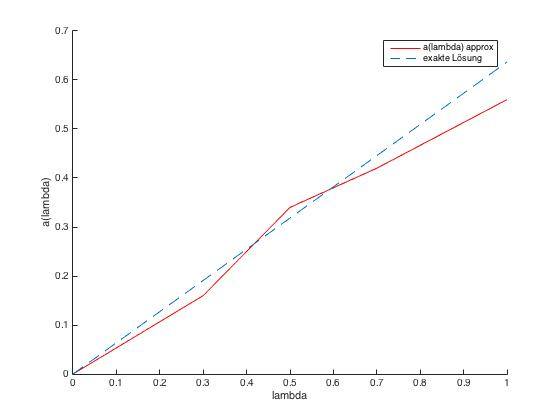
\includegraphics[width=12cm]{50.jpg}
%\caption{n=50} 
%\end{figure}

\begin{figure}[H]
\centering
%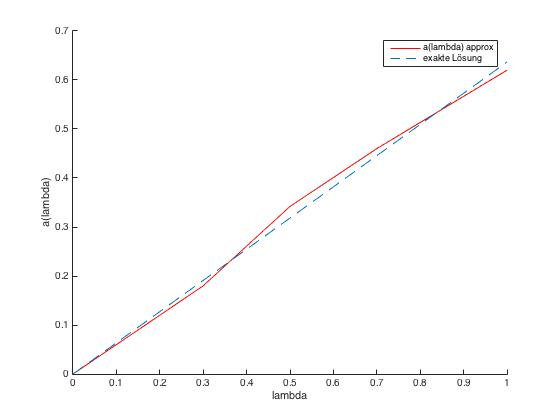
\includegraphics[width=12cm]{500.jpg}
%\caption{n=500}
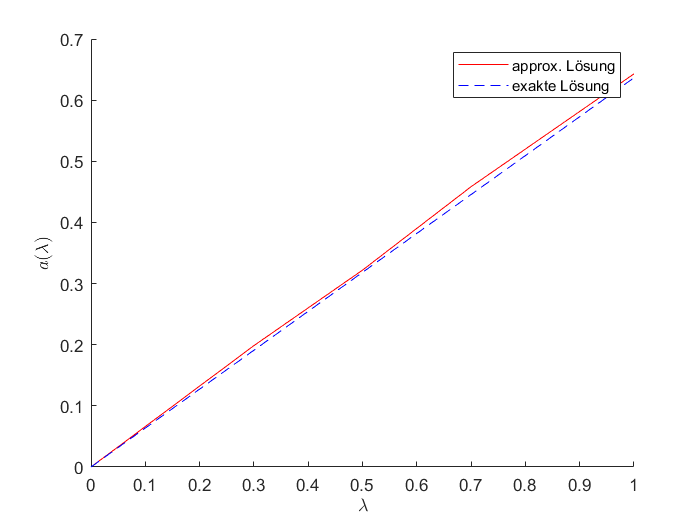
\includegraphics[width=12cm]{2000.png}
\caption{n=2000}
\end{figure}
Dies ist ein Plot mit den Ergebnissen aus obiger Tabelle und nur vier St"utzstellen.
Nun betrachten wir Plots mit einer gr"o"seren St"utzstellenanzahl. Genauer unterteilen wir das Intervall $[0,1]$ in $100$ gleichm"a"sig verteilte St"utzstellen.\\
Es ist zu erkennen, dass mit steigender Sampleanzahl das Ergenis deutlich besser wird und sich die Funktion der exakten L"osung $a(\lambda)$ ann"ahert.
\begin{figure}[H]
\centering
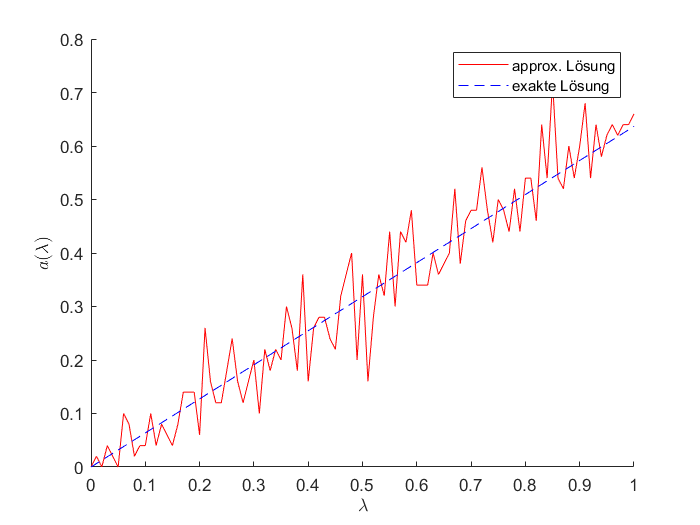
\includegraphics[width=12cm]{mc_n_50.png}
\caption{n=50}

\end{figure}
\begin{figure}[H]
\centering
%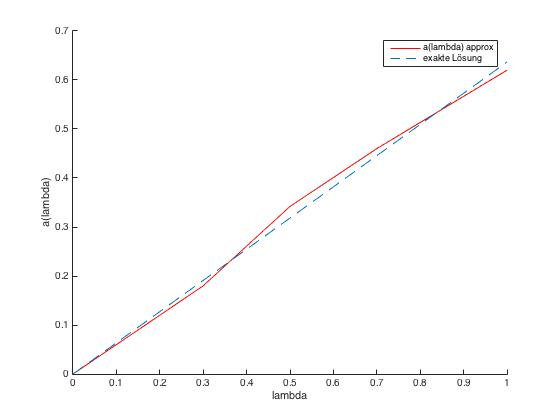
\includegraphics[width=12cm]{500.jpg}
%\caption{n=500}
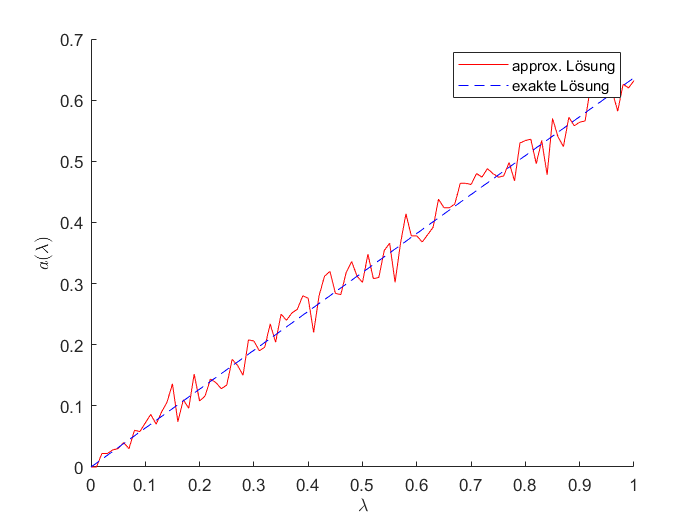
\includegraphics[width=12cm]{mc_n_500.png}
\caption{n=500}
\end{figure}

\begin{figure}[H]
\centering
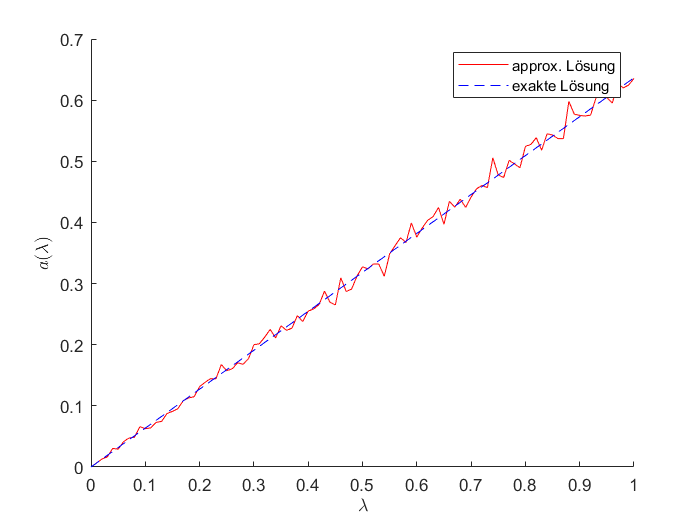
\includegraphics[width=12cm]{mc_n_2000.png}
\caption{n=2000}
\end{figure}





Mit steigender Sampleanzahl, d.h wiederholter Anzahl von Nadelw"urfen wird nat"urlich das Ergebnis besser bzw. genauer, da nach dem starken Gesetz der gro"sen Zahlen $\frac{1}{n}\sum_{i=1}^n X_i$ f"ur $n\rightarrow \infty$
fast sicher gegen $\mathbb{E}(X_1)$ konvergiert.%\vspace{1cm}

\begin{figure}[h]
\centering
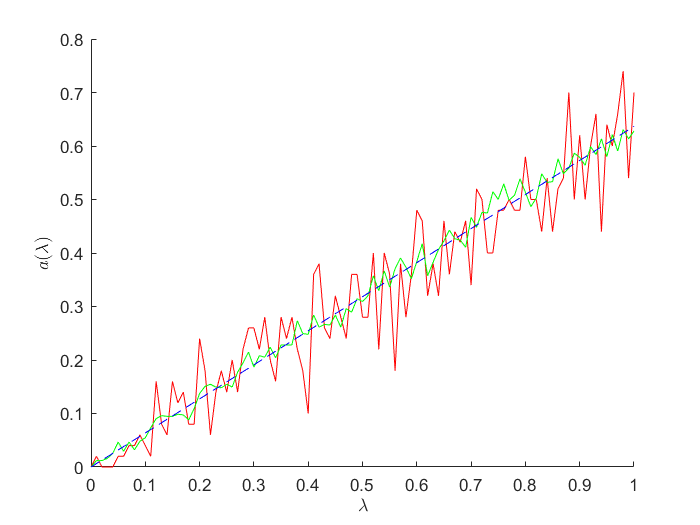
\includegraphics[width=12cm]{mc_n_50_gemittelt.png}
\caption{n=50 gemittelt}
\end{figure}

Bei obigem Plot beschreibt der gr"une Graph den Durchschnitt aus 15 Ausf"uhrungen an jeder St"utzstelle.\vspace{0.3cm}

Verwenden wir nun aber die Ergebnisse aus Proposition 3.1 Das bedeutet, wir geben uns eine Fehlerschranke $\varepsilon$ und $\theta$ vor und schauen, welches $L_\theta$ und welche Sampleanzahl uns geliefert werden. Die letzte Spalte der jeweiligen Tabellen enth"alt den tats"achlichen Fehler nach Gleichung (2).\\
Es ist in allen F"allen zu erkennen, dass der tats"achliche Fehler weit unter der vorgegebenen Schranke $\varepsilon$ liegt. Dies liegt daran, dass wir sowohl $L_\theta$ als auch $n_\theta$ aufrunden.
Weiterhin gilt nat"urlich, dass eine kleinere Fehlerschranke automatisch eine h"ohere Sampleanzahl und eine feinere Diskretisierung fordert.\\[0,2cm]
F"ur diese Tabelle gilt $\theta=0,3$.
\begin{center}
\begin{tabular}{c|c|c|c}
Fehlerschranke $\varepsilon$ & $n_\theta$ & $L_\theta$ & $\|a-\mathcal{M}_L^{\text{MC}}(n)\|_{L^2(\Omega,H)}$\\
\hline
$10^{-1}$  &  $2.81 \cdot 10^{1}$ &   $3$  &  $9.11 \cdot 10^{-3}$ \\
$10^{-2}$    & $2.63 \cdot 10^{3}$ &   $7$  &  $7.82 \cdot 10^{-5}$  \\
$10^{-3}$    & $2.62 \cdot 10^{5}$  &  $10$  &  $8.29 \cdot 10^{-7}$  \\
$10^{-4}$    &  $2.62 \cdot 10^{7}$ &   $13$  &  $9.01 \cdot 10^{-9}$ \\
$10^{-5}$ &   $2.62 \cdot 10^{9}$ &   $17$ &   $7.79 \cdot 10^{-11}$ \\
$10^{-6}$&   $2.62 \cdot 10^{11}$  &  $20$  &  $8.23 \cdot 10^{-13}$ \\ 
\hline 
 \end{tabular}
 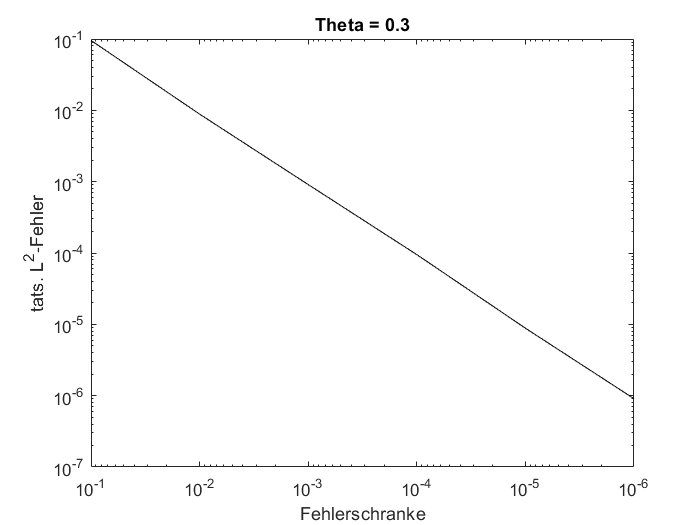
\includegraphics[width=12cm]{Plot1.png}
\end{center} 
\newpage
Hier gilt $\theta=0,5$.\\
\begin{center}
\begin{tabular}{c|c|c|c}
Fehlerschranke $\varepsilon$ & $n_\theta$ & $L_\theta$ & $\|a-\mathcal{M}_L^{\text{MC}}(n)\|_{L^2(\Omega,H)}$\\
\hline
$10^{-1}$  &  $3.93 \cdot 10^{1}$ &   $3$  &  $7.11 \cdot 10^{-3}$ \\
$10^{-2}$    & $3.7 \cdot 10^{3}$ &   $6$  &  $8.3 \cdot 10^{-5}$  \\
$10^{-3}$    & $3.67 \cdot 10^{5}$  &  $10$  &  $6.29 \cdot 10^{-7}$  \\
$10^{-4}$    &  $3.66 \cdot 10^{7}$ &   $13$  &  $7.01 \cdot 10^{-9}$ \\
$10^{-5}$ &   $3.66 \cdot 10^{9}$ &   $16$ &   $8.15 \cdot 10^{-11}$ \\
$10^{-6}$&   $3.66 \cdot 10^{11}$  &  $19$  &  $9.91 \cdot 10^{-13}$ \\ 
\hline 
 \end{tabular}\\
 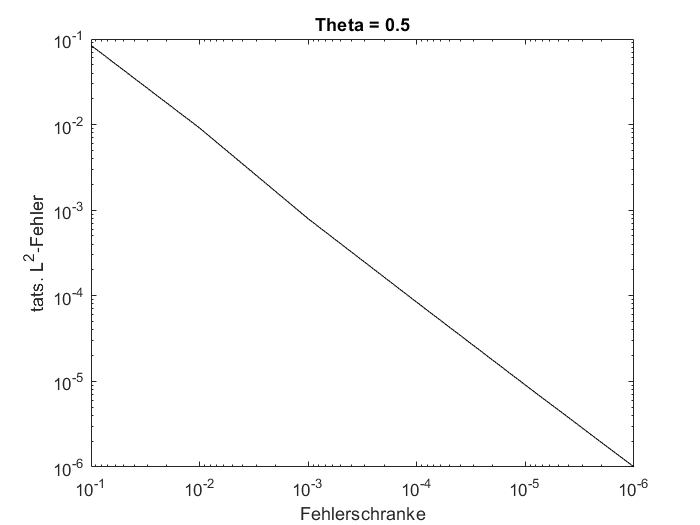
\includegraphics[width=14cm]{Plot2.png}
 \end{center}\newpage
Hier gilt $\theta=0,7$.
\begin{center}
\begin{tabular}{c|c|c|c}
Fehlerschranke $\varepsilon$ & $n_\theta$ & $L_\theta$ & $\|a-\mathcal{M}_L^{\text{MC}}(n)\|_{L^2(\Omega,H)}$\\
\hline
$10^{-1}$  &  $6.55 \cdot 10^{1}$ &   $3$  &  $5.11 \cdot 10^{-3}$ \\
$10^{-2}$    & $6.17 \cdot 10^{3}$ &   $6$  &  $6.3 \cdot 10^{-5}$  \\
$10^{-3}$    & $6.11 \cdot 10^{5}$  &  $9$  &  $8.15 \cdot 10^{-7}$  \\
$10^{-4}$    &  $6.1 \cdot 10^{7}$ &   $13$  &  $5.01 \cdot 10^{-9}$ \\
$10^{-5}$ &   $6.1 \cdot 10^{9}$ &   $16$ &   $6.15 \cdot 10^{-11}$ \\
$10^{-6}$&   $6.11 \cdot 10^{11}$  &  $19$  &  $7.91 \cdot 10^{-13}$ \\ 
\hline 
 \end{tabular}\\
 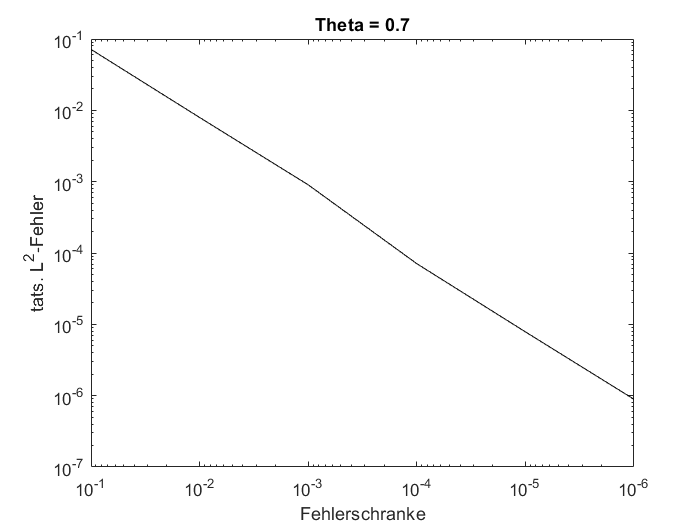
\includegraphics[width=14cm]{Plot3.png}
\end{center}


\newpage 
\section{Die Multi-Level-Monte-Carlo-Methode}
Die Multi-Level-Monte-Carlo-Methode (MLMC) beruht genauso wie die klassische Monte-Carlo-Methode auf wiederholtem zuf"alligem Sampling. Jedoch werden diese Samples nun auf unterschiedlichen Level von unterschiedlicher Genauigkeit ausgef"uhrt.
Die MLMC-Methode kann die Rechenkosten der klassischen MC-Methode stark reduzieren, indem man die meisten Samples auf einem Level mit niedriger Genauigkeit und entsprechend niedrigen Kosten nimmt und nur wenige Samples bei hoher Genauigkeit und entsprechend hohen Kosten.\\
Auch bei der MLMC-Methode ist das Ziel, die Erwartung $\mathbb{E}(X)$ einer Zufallsvariable $X$ zu approximieren. Dazu nutzt man  eine Folge von Approximationen $X_0,X_1,...,X_L$ mit ansteigender Genauigkeit und Kosten, die f"ur $L\longrightarrow\infty$ gegen $X$ konvergieren.\\
Die Grundlage der Multi-Level-Methode ist die Teleskopsumme. Genauer:
\begin{align*}
\mathbb{E}(X_L)=\mathbb{E}(X_0)+\sum_{l=1}^L \mathbb{E}(X_l-X_{l-1}).
\end{align*}
Durch die Linearit"at des Erwartungswertes ist diese Gleichung trivialerweise erf"ullt. Dabei wird jede Erwartung $\mathbb{E}(X_l-X_{l-1})$ durch die Monte-Carlo-Methode approximiert. Man muss jedoch beachten, dass ein Sample von $X_l-X_{l-1}$ auf dem Level $l$ sowohl eine Simulation von $X_{l-1}$ als auch von $X_l$ ben"otigt.\\
Die MLMC-Methode funktioniert, falls die Varianz $\text{Var}[X_l-X_{l-1}]$ f"ur $l\rightarrow\infty$ gegen $0$ konvergiert. Dies ist jedoch der Fall, falls $X_l$ und $X_{l-1}$ dieselbe Zufallsvariable approximieren.\vspace{1cm}

F"ur den MLMC-Algorithmus angewandt auf unser Nadelproblem definieren wir $D_0=Y_0$ und f"ur $l=1,2,...$
\begin{align*}
D_l(x,\alpha):=(Y_l-Y_{l-1})(x,\alpha)=\sum_{j=1}^{m_l} f(x,\alpha;\lambda_j^l)\mathbb{I}_{(\lambda_{j-1}^l,\lambda_j^l]}-\sum_{j=1}^{m_{l-1}}f(x,\alpha;\lambda_j^{l-1})\mathbb{I}_{(\lambda_{j-1}^{l-1},\lambda_j^{l-1}]}
\end{align*}
Zuerst betrachten wir die Varianz und den Erwartungswert von $D_l$.
\newpage
\begin{prop}\label{k}
Es gilt $\mathbb{E}(D_0)=a(1)\mathbb{I}_{(0,1]}$ und f"ur jedes $l=1,2,...$ gilt
\begin{align*}
\mathbb{E}(D_l)=\sum_{j=1}^{m_{l-1}}(a(\lambda_{2j-1}^l)-a(\lambda_{2j}^l))\mathbb{I}_{(\lambda_{2j-2}^l,\lambda_{2j-1}^l]}.
\end{align*}
Zus"atzlich gilt f"ur alle $l\in\mathbb{N}$
\begin{align*}
\|D_l-\mathbb{E}[D_l]\|^2_{L^2(\Omega,H)}=\frac{1}{\pi m_l}\left(1-\frac{2}{\pi m_l}\right).
\end{align*}
\end{prop}
\begin{proof}
Es gilt $\lambda_{j-1}^{l-1}=\frac{j-1}{2^{l-1}}=\frac{2(j-1)}{2^l}=\lambda^l_{2(j-1)}$ und analog $\lambda_j^{l-1}=\lambda_{2j}^l$.\\
Deshalb gilt auch 
\begin{align*}
\mathbb{I}_{(\lambda_{j-1}^{l-1},\lambda_j^{l-1}]}=\mathbb{I}_{(\lambda_{2(j-1)}^{l},\lambda_{2j}^{l}]}=\mathbb{I}_{(\lambda_{2(j-1)}^{l},\lambda_{2j-1}^{l}]}+\mathbb{I}_{(\lambda_{2j-1}^{l},\lambda_{2j}^{l}]} 
\end{align*}
f"ur alle $ l=1,2,...$ und $ j=1,...,m_l$.\\
Damit folgt
\begin{align*}
\mathbb{E}[D_l]=&\mathbb{E}\left(\sum_{j=1}^{m_l}f(x,\alpha;\lambda_j^l)\mathbb{I}_{(\lambda_{j-1}^{l},\lambda_j^{l}]}\right)-\mathbb{E}\left(\sum_{j=1}^{m_{l-1}}f(x,\alpha;\lambda_j^{l-1})\mathbb{I}_{(\lambda_{j-1}^{l-1},\lambda_j^{l-1}]}\right)\\=&\sum_{j=1}^{m_l}a(\lambda_j^l)\mathbb{I}_{(\lambda_{j-1}^{l},\lambda_j^{l}]}-\sum_{j=1}^{m_{l-1}}a(\lambda_j^{l-1})\mathbb{I}_{(\lambda_{j-1}^{l-1},\lambda_j^{l-1}]}\\=&\sum_{j=1}^{m_{l-1}}\left(a(\lambda_{2j-1}^l)\mathbb{I}_{(\lambda_{2j-2}^{l},\lambda_{2j-1}^{l}]}+a(\lambda_{2j}^l)\mathbb{I}_{(\lambda_{2j-1}^{l},\lambda_{2j}^{l}]}\right)\\-&\sum_{j=1}^{m_{l-1}}\left(a(\lambda_{j}^{l-1})\mathbb{I}_{(\lambda_{2(j-1)}^{l},\lambda_{2j-1}^{l}]}+a(\lambda_{j}^{l-1})\mathbb{I}_{(\lambda_{2j-1}^{l},\lambda_{2j}^{l}]}\right)\\=& \sum_{j=1}^{m_{l-1}}a(\lambda_{2j-1}^l)-a(\lambda_{2j}^l))\mathbb{I}_{(\lambda^l_{2j-2},\lambda^l_{2j-1}]}=\sum_{j=1}^{m_l}\left(-\frac{2}{\pi m_l}\right)\mathbb{I}_{(\lambda^l_{2j-2},\lambda^l_{2j-1}]}.
\end{align*}
Dies beweist den ersten Teil der Proposition. F"ur den zweiten Teil gilt
\allowdisplaybreaks
\begin{align*}
\|D_l-\mathbb{E}(D_l)\|^2_{L^2(\Omega,H)}
=&\mathbb{E}
\int_0^1|\sum_{j=1}^{m_l}
f(\cdot;\lambda_j^l)\mathbb{I}_{(\lambda_{j-1}^l,\lambda_j^l]}
\sum_{j=1}^{m_{l-1}}f(\cdot;\lambda_j^{l-1})\mathbb{I}_{(\lambda_{j-1}^{l-1},\lambda_j^{l-1}]}\\
-&\sum_{j=1}^{m_{l-1}}\left(-\frac{2}{\pi m_l}\right)\mathbb{I}_{(\lambda^l_{2j-2},\lambda^l_{2j-1}]}|^2\td{\lambda}\\
=&\mathbb{E}\int_0^1|\sum_{j=1}^{m_{l-1}}f(\cdot;\lambda_{2j-1}^{l})-f(\cdot;\lambda_{2j}^{l})+\frac{2}{\pi m_l})\mathbb{I}_{(\lambda^l_{2j-2},\lambda^l_{2j-1}]}|^2\td{\lambda}\\
=& \sum_{j=1}^{m_{l-1}}\frac{1}{m_l}\left(\mathbb{E}|f(\cdot;\lambda^l_{2j-1})-f(\cdot;\lambda_{2j}^l)|^2-\left(\frac{2}{\pi m_l}\right)^2\right)\\
=&\frac{1}{m_l}\sum_{j=1}^{m_{l-1}}\frac{2}{\pi m_l}\left(1-\frac{2}{\pi m_l}\right)=\frac{1}{m_l}\left(m_{l-1}\left(\frac{2}{\pi m_l}\left(1-\frac{2}{\pi m_l}\right)\right)\right)
\\=&
\frac{1}{\pi m_l}\left(1-\frac{2}{\pi m_l}\right),
\end{align*}
da $\frac{m_{l-1}}{m_l}=\frac{1}{2}$.
\end{proof}


\subsection{Implementierung der Multi-Level-Monte-Carlo-Methode}
Meinem Programm wird ein Vektor $n$ einer bestimmen L"ange $L$ "ubergeben. Diese L"ange $L$ entspricht der Anzahl der Level. $n(i)$ ist die Anzahl an Samples im jeweiligen Level $i$.
In folgenden Tabellen sind die Ergebnisse f"ur unterschiedliche $\lambda$ und zugeh"origem Vektor $n$ eingetragen. Es ist wieder zu erkennen, dass das Ergebnis stark von der Anzahl der Samples und Level abh"angt. In diesem Kapitel habe ich nur zuf"allig eine Levelanzahl und die zugeh"origen Sampleanzahlen gew"ahlt, um erste Ergebnisse zu sehen. Nat"urlich unter der Voraussetzung, dass die Sampleanzahl mit steigendem Level sinkt. Sp"ater wird dies organisierter geschehen. \\[0.5cm]

 $n=[2000,1000,700,600,500,400,300,100,50]$, Anzahl Level = 9:
\begin{center}
\begin{tabular}{l|c|c|c|c|c|c|c|r}
 $\lambda$&0& $0.1$&$0.2$&$0.3$&$0.5$.&$0.7$&$0.8$&$1$\\
 \hline
 $a(\lambda)$&0   & 0.1329   & 0.1912   & 0.2168  &  0.3605 &   0.4402  &  0.5372  &  0.6495 \\ 
 \hline 
 \end{tabular}
  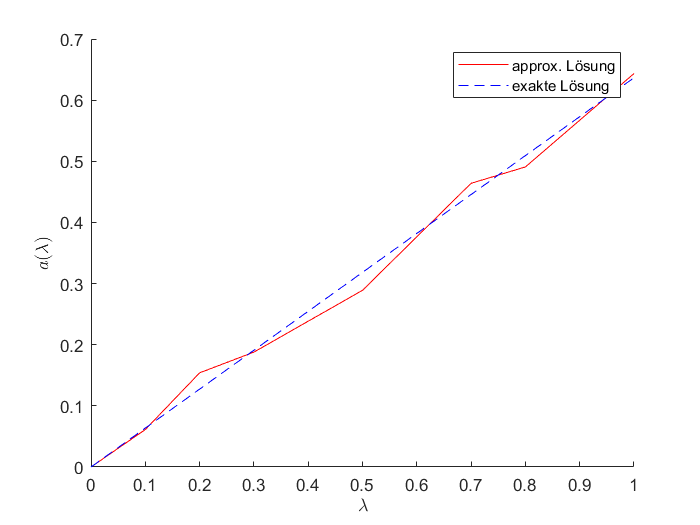
\includegraphics[width=11cm]{MLMC1.png}
 \end{center}\newpage
$n= [5000,4000,3000,2000,1000,700,600,500]$, Anzahl Level = 8,\\
\begin{center}
\begin{tabular}{l|c|c|c|c|c|c|c|r}
 $\lambda$&0& $0.1$&$0.2$&$0.3$&$0.5$.&$0.7$&$0.8$&$1$\\
 \hline
 $a(\lambda)$&0 &   0.0783 &   0.1479 &   0.2261 &   0.3372  &  0.4532  &  0.5229 &   0.6434 \\ 
 \hline 
 \end{tabular}
  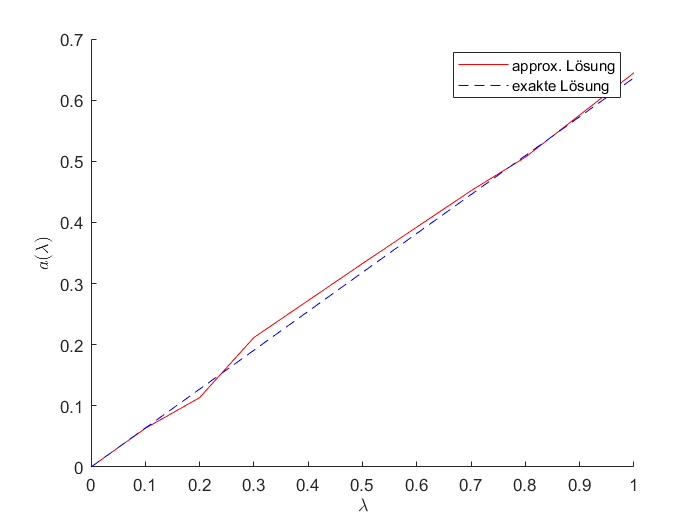
\includegraphics[width=11cm]{MLMC2.png}
 \end{center}
 Das Ergebnis ist trotz kleinerer Levelanzahl besser, da deutlich mehr Samples auf den jeweiligen Leveln genommen wurden.\vspace{0,5cm}
 
$n= [10000,8000,6000,4000,3000,2000,1000,600,500,100,50]$, Anzahl Level = 11:
 \begin{center}
\begin{tabular}{l|c|c|c|c|c|c|c|r}
 $\lambda$&0& $0.1$&$0.2$&$0.3$&$0.5$.&$0.7$&$0.8$&$1$\\
 \hline
 $a(\lambda)$& 0  &  0.0648  &  0.1255 &   0.1935  &  0.3158 &   0.4452 &   0.5074 &   0.6357\\ 
 \hline 
 \end{tabular}
  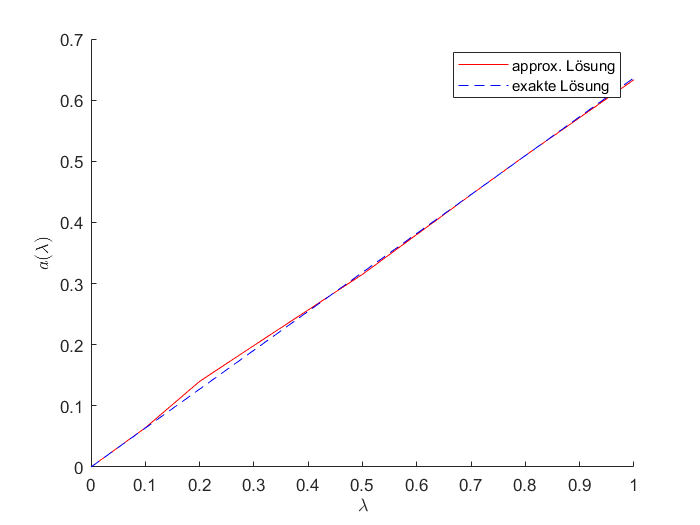
\includegraphics[width=11cm]{MLMC3.png}
 \end{center}\vspace{1cm}


\subsection{Einschub: Zufallsvariablen mit Werten in Banachr"aumen}
F"ur die Fehleranalyse der Multi-Level-Monte-Carlo-Methode ben"otigen wir einige neue Definitionen von Zufallsvariablen, die ihre Werte in Banachr"aumen haben. In diesem Kapitel folgen wir \cite{Heinrich} und geben einen kurzen "Uberblick "uber die zugeh"orige Integrationstheorie.\\[0,2cm]

Es sei $E$ ein $\mathbb{R}$-Banachraum mit Norm $\|\cdot\|$. $\mathcal{B}(E)$ bezeichne die Borel-$\sigma$-Algebra, welche durch die offenen Mengen in $E$ erzeugt wird. Au"serdem sei $(\Omega,\mathcal{F},\mathbb{P})$ ein vollst"andiger Wahrscheinlichkeitsraum.

\begin{df}
Eine Abbildung $X:\Omega\rightarrow E$ hei"st eine \textbf{$E$-wertige Zufallsvariable}, falls $X$ $\mathcal{F}-\mathcal{B}(E)$-messbar ist.\\
Falls es eine $\mathbb{P}$-Nullmenge $\mathcal{N}\in\mathcal{F}$ gibt,  mit $X(\mathcal{N}^c)\subset E$ seperabel, dann nennen wir $X$ \textbf{stark messbar}. Die Menge aller stark messbaren Zufallsvariablen, welche Werte in E annehmen, werden mit $\mathcal{L}^0(\Omega,\mathcal{F},\mathbb{P};E)$ bezeichnet.
\end{df}

\begin{df}
Es sei $1\leq p <\infty$. Eine stark messbare Zufallsvariable $X \in \mathcal{L}^0(\Omega,\mathcal{F},\mathbb{P};E)$ hei"st \textbf{p-fach integrierbar}, falls gilt
\begin{align*}
\|X\|_{L^p(\Omega,E)}:=(\mathbb{E}[\|X\|^p])^{\frac{1}{p}}:=\left(\int_\Omega \|X(\omega)\|^p \text{d}\mathbb{P}(\omega)\right)^{\frac{1}{p}}<\infty.
\end{align*}
Die Menge aller p-fach integrierbaren Zufallsvariablen mit Werten in E wird mit $\mathcal{L}^p(\Omega,\mathcal{F},\mathbb{P};E)$ bezeichnet.
\end{df}
Im Allgemeinen definiert die Abbildung $\|\cdot\|_{L^p{(\Omega,E)}}:\mathcal{L}^p(\Omega,\mathcal{F},\mathbb{P};E)\rightarrow \mathbb{R}$ nur eine Halbnorm.
Wie "ublich identifiziert man Zufallsvariablen miteinander, die $\mathbb{P}$-fast sicher "ubereinstimmen. Das bedeutet $X\sim Y \Leftrightarrow \|X-Y\|_{L^p(\Omega,E)}=0$ f"ur $1\leq p<\infty$.\\
Die Lebesgue-R"aume $L^p(\Omega,E):=L^p(\Omega,\mathcal{F},\mathbb{P};E):=\mathcal{L}^p(\Omega,\mathcal{F},\mathbb{P};E)/\sim$ werden zu Banachr"aumen, falls sie mit der Norm $\|\cdot\|_{L^p(\Omega,E)}$ f"ur $1\leq p < \infty$ versehen werden.
Falls $E$ ein Hilbertraum mit Skalarprodukt $\langle\cdot,\cdot\rangle$ ist, dann ist $L^2(\Omega;E)$ auch ein Hilbertraum mit Skalarprodukt
\begin{align*}
\langle X,Y \rangle_{L^2(\Omega,E)}:=\mathbb{E}[\langle X,Y \rangle_E]:=\int_\Omega \langle X(\omega),Y(\omega) \rangle_E \text{d}\mathbb{P}(\omega).
\end{align*}
Die Konstruktion des Bochner-Lebesgue-Integrals verl"auft wie gewohnt.\\
Zuerst betrachten wir einfache Zufallsvariablen, welche nur endlich viele Werte in E annehmen. Das bedeutet $X=\sum_{j=1}^n \mathbb{I}_{A_j}e_j$ f"ur $n\in\mathbb{N},(e_j)_{j=1}^n\subset E\setminus\{0\}$ und $(A_j)_{j=1}^n\subset \mathcal{F}$ mit $e_j\neq e_i$ und $A_j \cap A_i = \emptyset$ falls $j\neq i$.\\
\begin{df}[Bochner-Lebesgue-Integral]
Das \textbf{Bochner-Lebesgue-Integral} ist definiert durch
\begin{align*}
\mathbb{E}[X]:=\int_\Omega X(\omega)\text{d}P(\omega):=\sum_{j=1}^n\mathbb{P}(A_j)e_j\in E.
\end{align*}
\end{df}
Diese Definition h"angt nicht von einer bestimmten Darstellung von $X$ ab. Ferner ist die Erwartung eine lineare Abbildung vom Raum aller einfachen Zufallsvariablen in $E$ und es gilt $\|\mathbb{E}[X]\|\leq\|X\|_{L^1(\Omega;E)}$ f"ur jedes einfache $X:\Omega\rightarrow E.$\\[0,1cm]
Die Definition von $\mathbb{E}[\cdot]$ kann auf den Abschluss der Menge der einfachen Zufallsvariablen bzgl. der $L^1$-Norm erweitert werden. Tats"achlich folgt aus der Eigenschaft der Separabilit"at, dass f"ur jedes $X\in\mathcal{L}^1(\Omega,\mathcal{F},\mathbb{P};E)$ eine Folge von einfachen Zufallsvariablen $(X_n)_{n\in\mathbb{N}}$ existiert, sodass $\lim_{n\rightarrow \infty}\|X-X_n\|_{L^1(\Omega;E)}=0$.\\
Die Erwartung von $X$ ist dann definiert durch,
\begin{align*}
\mathbb{E}[X]:=\int_\Omega X(\omega)\text{d}\mathbb{P}(\omega):=\lim_{n\rightarrow \infty} \mathbb{E}[X_n]\in E.
\end{align*}
Das Element $\mathbb{E}[X]$ h"angt nicht von der Wahl der Folge $(X_n)_{n\in\mathbb{N}}$ ab. Es gilt $\mathbb{E}[X]=\mathbb{E}[Y]$, falls $X=Y$ fast sicher gilt. \\
Daher ist das Bochner-Lebesgue-Integral eine lineare Abbildung $\mathbb{E}[\cdot]:L^1(\Omega;E)\rightarrow E$, welche $\|\mathbb{E}[X]\|_E\leq \|X\|_{L^1(\Omega;E)}$ erf"ullt.\\
Es gibt offenbar keinen gro"sen Unterschied zwischen der Erwartung einer reellen Zufallsvariable und einer welche ihre Werte in einem Banachraum annimmt. Jedoch gilt nicht mehr die Formel von Bienayme. Diese Formel hat keine direktes Gegenst"uck f"ur Zufallsvariablen mit Werten in Banachr"aumen. Um dieses Problem zu umgehen beschr"anken wir uns auf Banachr"aume mit folgender Eigenschaft.
\begin{df}
Sei $(\varepsilon_i)_{i\in\mathbb{N}}$ eine \textbf{Rademacher-Folge}. 
Das hei"st $(\varepsilon_i)_{i\in\mathbb{N}}$ ist eine Folge von reellwertigen unabh"angig und identisch verteilten Zufallsvariablen auf $\Omega$ mit $\mathbb{P}(\varepsilon_i=\pm 1)=\frac{1}{2}$ f"ur jedes $i\in\mathbb{N}$.\\
Wir sagen ein Banachraum $E$ ist von \textbf{Rademacher-Typ $p\in [1,2]$}, falls es eine Konstante $C$ gibt, sodass 
\begin{align*}
\Big\|\sum_{i=1}^n \varepsilon_i e_i \Big\|_{L^p(\Omega;E)}\leq C \left(\sum_{i=1}^n\|e_i\|^p\right)^{\frac{1}{p}}
\end{align*}
f"ur alle $n\in\mathbb{N}$ und jede endliche Folge $(e_i)_{i=1}^n\subset E$ gilt. Das minimale $C$ wird \textbf{Typ-p-Konstante} von E genannt und wird mit $T_p(E)$ bezeichnet.
\end{df}
\begin{bsp}
\begin{enumerate}
\item[a)]Durch die Dreiecksungleichung folgt, dass jeder Banachraum von Typ $p=1$ ist.
\item[b)]Jeder Hilbertraum ist von Typ $p=2$. In diesem Fall gilt sogar Gleichheit mit $T_2(E)=1$.
Da es sich bei  $L^2(\Omega,H)$ um einen Hilbertraum handelt, gilt in diesem Fall also $p=2$ und $T_2(E)=1$.
\end{enumerate}
\end{bsp}
Folgende Proposition "ubernimmt die Rolle der Formel von Bienayme in den folgenden Kapiteln.
\begin{prop}\label{Ung}
Sei $p\in [1,2]$ und $E$ ein Banachraum von Typ p. Dann gilt f"ur jede endliche Folge $(X_i)^n_{i=1}\subset L^p(\Omega;E),n\in \mathbb{N}$, von unabh"angigen Zufallsvariablen mit $\mathbb{E}[X_i]=0$
\begin{align*}
\mathbb{E}\left[\Big\|\sum_{i=1}^nX_i\Big\|^p\right]\leq (2T_p(E))^p\sum_{i=1}^n\mathbb{E}[\|X_i\|^p].
\end{align*}
\end{prop}
\begin{proof}
siehe \cite{Heinrich}.
\end{proof}
\newpage
\subsection{Fehlerschranken f"ur die MLMC-Methode}
In diesem Kapitel formulieren wir die MLMC-Methode allgemein f"ur Zufallsvariablen, die ihre Werte in Banachr"aumen haben.
Es sei $p\in (1,2]$ und $E$ ein $\mathbb{R}$-Banachraum von Typ $p$. Wir werden eine
Sch"atzung des Fehlers bez"uglich der Norm in $L^p(\Omega;E)$ erhalten.\\
Unser Ziel ist die Approximation von
\begin{align*}
a=\mathbb{E}(Y)\in E,
\end{align*}
wobei $Y\in L^p(\Omega;E)$ eine gegebene Zufallsvariable ist.\\
Hierf"ur nehmen wir an, dass eine Folge $(D_l)_{l\in\mathbb{N}}\subset L^p(\Omega;E)$ von unabh"angigen und identisch verteilten Zufallsvariablen existiert,welche folgende Eigenschaften erf"ullt:\\[0,1cm]
F"ur $L\in \mathbb{N}$ sei
\begin{align*}
Y_L:=\sum_{l=1}^L D_l;
\end{align*}
oder "aquivalent hierzu
\begin{align*}
Y_l=Y_{l-1}+D_l, \ \ l\in\mathbb{N}
\end{align*}
mit $Y_0:=0\in L^p(\Omega;E).$ Nun fordern wir, dass gilt
\begin{itemize}
\item[(A)]$\lim_{L\in \mathbb{N}}\|a-\mathbb{E}[Y_L]\|=0$;
\item[(B)]$\sup_{L\in\mathbb{N}}\|Y_L-\mathbb{E}[Y_L]\|_{L^p(\Omega;E)}<\infty.$
\end{itemize}
Die Forderung (A) gew"ahrleistet, dass die statistische Abweichung zwischen $Y_L$ und $a$ f"ur $L\rightarrow \infty$ klein wird und (B) gibt uns  Kontrolle "uber die $L^p$-Norm von $Y_L$.\\
Zusammen jedoch sind beide Bedingungen n"utzlich um zu gew"ahrleisten, dass die klassische MC-Methode bzgl. der $L^p(\Omega;E)$-Norm gegen $a\in E$ konvergiert. \\
Sei nun also $(Y_{L,i})_{i\in\mathbb{N}}$ eine Folge von unabh"angigen und identisch verteilten Kopien von $Y_L$, dann folgt mit \ref{Ung}, dass 
\begin{align*}
\Big\|a-\frac{1}{n}\sum_{i=1}^nY_{L,i}\Big\|_{L^p(\Omega;E)}\leq
\| a-\mathbb{E}[Y_L]\|_{L^p(\Omega,E)}+\frac{2T_p(E)}{n^{1-\frac{1}{p}}}\cdot\|Y_L-\mathbb{E}[Y_L]\|_{L^p(\Omega;E)}.
\end{align*} gilt.
Dies folgt wegen
\begin{align*}
\left \|a-\frac{1}{n}\sum_{i=1}^nY_{L,i}\right \|_{L^p(\Omega,E)}\leq\left\|a-\mathbb{E}(Y_L)\right\|_{L^p(\Omega,E)}+\left\|\mathbb{E}(Y_L)-\frac{1}{n}\sum_{i=1}^nY_{L,i}\right\|_{L^p(\Omega,E)}
\end{align*}
und es ist 
\begin{align*}
\left\| \mathbb{E}(Y_L)-\frac{1}{n}\sum_{i=1}^n Y_{L,i}\right\|_{L^p(\Omega,E)}
=&\left\|\frac{1}{n}\sum_{i=1}^n(\mathbb{E}(Y_L)-Y_{L,i})
\right\|_{L^p(\Omega,E)}\\ \stackrel{4.6}{\leq}& 2T_p(E) \left(\frac{1}{n^p}\sum_{i=1}^n \| \mathbb{E}(Y_L)-Y_{L,i}\|_{L^p(\Omega,E)}\right)^{\frac{1}{p}}\\
\overset{(*)}{=}&2T_p(E)\left(\frac{1}{n^{p-1}}\|\mathbb{E}(Y_L)-Y_L\|^p_{L^p(\Omega,E)}\right)^{\frac{1}{p}}\\
=&2T_p(E)\frac{1}{n^{1-\frac{1}{p}}}\|\mathbb{E}(Y_L)-Y_L\|_{L^p(\Omega,E)}.
\end{align*}
Dabei gilt $(*)$, da $Y_{l,i}$ identisch verteilte Kopien von $Y_L$ sind.\\
Durch (A) und (B) wird die rechte Seite klein f"ur $L,n\rightarrow \infty$. Da $E$ unendlich dimensional sein kann und man sicher gehen will, dass die Approximation funktioniert, ist es sinnvoll zu verlangen, dass $Y_L$ nur Werte in einem endlich dimensionalen Unterraum von $E$ annimmt. Dies sollte man beachten, wenn man die zu approximierenden Folgen $(D_l)_{l_\in\mathbb{N}}$ und $(Y_l)_{l\in\mathbb{N}}$ von Zufallsvariablen konstruiert.\\[1cm]
Bez"uglich $(D_l)_{l\in\mathbb{N}}$ betrachten wir nun den MLMC-Sch"atzer:
Es sei $L\in\mathbb{N}$ und $(n_i)_{i=1}^l\subset \mathbb{N}$ gegeben. $(D_{l,i})_{i\in\mathbb{N}}$ sei eine Folge von unabh"angingen und identisch verteilten Kopien von $(D_l)_{l\in\mathbb{N}}$, so dass $(D_{l,i})_{l,i \in\mathbb{N}}\subset L^p(\Omega;E)$ eine Familie von unabh"angigen Zufallsvariablen bzgl. beider Parameter bildet. Dann ist der MLMC-Sch"atzer gegeben durch
\begin{align*}
\mathcal{M}_L^{\text{MLMC}}((n_l)_{l=1}^L):=\sum_{l=1}^L\frac{1}{n_l}\sum_{i=1}^{n_l}D_{l,i},
\end{align*} wobei $D_0=Y_0=0$ ist.
Offensichtlich gilt $\mathcal{M}_L^{\text{MLMC}}((n_l)_{l=1}^L)\in L^p(\Omega;E).$\\
W"ahrend die Fehleranalyse der klassischen MC-Methode mit den zwei obigen Eigenschaften der Folge $(Y_l)_{l\in\mathbb{N}}$ erfolgt, ist es f"ur die MLMC-Methode praktischer direkt folgende Bedingungen an die Folge $(D_l)_{l\in\mathbb{N}}\subset L^p(\Omega;E)$ zu stellen.
\begin{vor}
Sei $h\in(0,1)$ ein gegebener Wert, sodass die folgenden Bedingungen erf"ullt sind:
\begin{enumerate}
\item[a)] Es exisitiert eine Konstante $C_1$ und ein $q_1\in (0,\infty)$, sodass
\begin{align*}
\Big\|a-\mathbb{E}\left[\sum_{l=1}^L D_l \right]\Big\|\leq C_1h^{q_1L}
\end{align*}
f"ur alle $L\in\mathbb{N}$ gilt. Wir nennen $q_1$ die \textbf{schwache Konvergenzordnung}.
\item[b)] Es gibt eine Konstante $C_2$ und ein $q_2\in(0,\infty)$, sodass
\begin{align*}
\|D_l-\mathbb{E}[D_l]\|_{L^p(\Omega;E)}\leq C_2h^{q_2 l}
\end{align*}
f"ur alle $L\in\mathbb{N}$ gilt. Wir nennen $q_2$ die \textbf{starke Konvergenzordnung}.
\end{enumerate}
\end{vor}
Beide Teile a) und b) aus obiger Definition implizieren die zugeh"origen Bedingungen (A) und (B) an $(Y_l)_{l\in\mathbb{N}}$.
Da $h\in(0,1)$  und damit
\begin{align*}
\Big\|a-\mathbb{E}[\underbrace{\sum_{l=1}^L D_l }_{Y_L}]\Big\|\leq C_1h^{q_1L}\underset{L\rightarrow \infty}{\longrightarrow} 0
\end{align*}
folgt (A) direkt aus a).\\
Die Forderung (B) folgt aus der Dreiecksungleichung:
\begin{align*}
\|Y_L-\mathbb{E}[Y_L]\|_{L^p(\Omega;E)}=\|\sum_{l=1}^L(D_l-\mathbb{E}[D_l])\|_{L^p(\Omega;E)}\underset{b)}{\leq}\sum_{l=1}^L C_2 h^{q_2 l}\leq C_2 \cdot \sum_{l=1}^\infty(h^{q_2})^l= C_2(1-h^{q_2})^{-1}<\infty.
\end{align*}
Vergleichen wir Voraussetzung 4.7 mit Proposition 2.1 erhalten wir wegen  $\|a-\mathbb{E}(\sum_{l=1}^L D_l)\|=\|a-\mathbb{E}(Y_L)\|$ f"ur unser Buffonsches Nadelproblem die Konstanten $h,C_1$ und $q_1$. Proposition 2.1 besagt, dass f"ur alle $l\in\mathbb{N}_0$ 
\begin{align*}
\|a-\mathbb{E}(Y_l)\|_H=\frac{2}{\pi\sqrt{3}}\frac{1}{m_l}=\frac{2}{\pi\sqrt{3}}\left(\frac{1}{2}\right)^l\leq C_1h^{q_1l}
\end{align*} gilt.
Daraus folgt $h=\frac{1}{2}, q_1=1$ und $C_1=\frac{2}{\pi\sqrt{3}}$.\\[0,2cm]
Die Proposition \eqref{k} liefert $\|D_l-\mathbb{E}[D_l]\|^2_{L^2(\Omega,H)}=\frac{1}{\pi m_l}\left(1-\frac{2}{\pi m_l}\right)$.
Dadurch erhalten wir
\begin{align*}
\|D_l-\mathbb{E}[D_l]\|_{L^2(\Omega,H)}=\sqrt{\frac{1}{\pi m_l}\left(1-\frac{2}{\pi m_l}\right)}\leq \frac{1}{\pi m_l}\left(1-\frac{2}{\pi m_l}\right) \leq \frac{1}{\pi}\left(\frac{1}{2}\right)^l\leq C_2h^{q_2l},
\end{align*}
woraus $ q_2=1, C_2=\frac{1}{\pi}$ und $h=\frac{1}{2}$ folgt.


\begin{prop}
F"ur jede Wahl von $L\in\mathbb{N}$ und $(n_l)_{l=1}^L\subset\mathbb{N}$ gilt
\begin{align}\label{b}
\|a-\mathcal{M}_L^{\text{MLMC}}((n_l)_{l=1}^L)\|_{L^p(\Omega;E)}\leq\|a-a_L\|+2T_p(E)\left(\sum_{l=1}^L\frac{1}{n_l^{p-1}}\|D_l-\mathbb{E}[D_l]\|^p_{L^p(\Omega;E)}\right)^{\frac{1}{p}},
\end{align}
mit $a_L=\sum_{l=1}^L\mathbb{E}[D_l]$. Falls $(D_l)_{l\in\mathbb{N}}$ a) und b) aus obiger Definition erf"ullt, dann folgt
\begin{align}\label{c}
\|a-\mathcal{M}_L^{\text{MLMC}}((n_l)_{l=1}^L)\|_{L^p(\Omega;E)}\leq C_1 h^{q_1L}+2C_2 T_p(E)\left(\sum_{l=1}^L \frac{h^{p q_2 l}}{n_l^{p-1}}\right)^{\frac{1}{p}}.
\end{align}
\end{prop}
\begin{proof}
Durch Einsetzen von $a_L$ und $\mathcal{M}_L^{\text{MLMC}}((n_l)_{l=1}^L$, liefert die Dreiecksungleichung
\begin{align*}
\|a-\mathcal{M}_L^{\text{MLMC}}((n_l)_{l=1}^L)\|_{L^p(\Omega;E)}\leq&
\|a-a_L\|+\|a_L-\mathcal{M}_L^{\text{MLMC}}((n_l)_{l=1}^L)\|_{L^p(\Omega;E)}\\
=&\|a-a_L\|+\left\|\sum_{l=1}^L \frac{1}{n_l}\sum_{i=1}^{n_l}(D_{l,i}-\mathbb{E}[D_l])\right\|_{L^p(\Omega;E)}.
\end{align*}
Nach Definition ist $(\frac{1}{n_l}(D_{l,i}-\mathbb{E}[D_l]))_{l,i\in\mathbb{N}}$ eine Familie von unabh"angigen zentrierten Zufallsvariablen. Deshalb k"onnen wir \ref{Ung} anwenden und erhalten
\begin{align*}
\Big\|\sum_{l=1}^L \frac{1}{n_l}\sum_{i=1}^{n_l}(D_{l,i}-\mathbb{E}[D_l])\Big\|_{L^p(\Omega;E)}\leq&\ 2T_p(E)\left(\sum_{l=1}^L\frac{1}{{n_l}^p}\sum_{i=1}^{n_l} \| D_{l,i}-\mathbb{E}[D_l]\|^p_{L^p(\Omega,E)}\right)^{\frac{1}{p}}\\
=& 2T_p(E)\left(\sum_{l=1}^L\frac{1}{{n_l}^{p-1}} \| D_{l}-\mathbb{E}[D_l]\|^p_{L^p(\Omega,E)}\right)^{\frac{1}{p}},
\end{align*}
da $(D_{l,i})_{l,i\in\mathbb{N}}$  identisch verteilte Kopien von $D_l$ sind. Dies beweist \eqref{b}. Wenden wir nun b) aus der Definition an, erhalten wir den zweiten Teil der Proposition \eqref{c}.
\end{proof}
\newpage 
\thispagestyle{empty}
\quad  
\newpage
\section{Optimierung der Parameter und des Rechenaufwandes der MLMC-Methode}
In diesem Kapitel besch"aftigen wir uns mit folgender Frage:\\
Sei $\varepsilon>0$ eine gegebene Fehlertoleranz.\\ Wie sind die Parameter $L\in \mathbb{N}$ (Anzahl der Level) und $(n_l)^L_{l=1}$ (Anzahl der Samples pro Level) in der MLMC-Methode zu w"ahlen, sodass der Rechenaufwand minimiert wird?\\
 Dies jedoch unter der Bedingung, dass der Fehler in \eqref{c} durch $\varepsilon$ beschr"ankt ist.\\
 Desweiteren wollen wir wissen, wie der Rechenaufwand von der Fehlertoleranz abh"angt, falls $\varepsilon\rightarrow 0$ gilt.\\
 Um diese Fragen zu beantworten, m"ussen wir zuerst festlegen, wie die Rechenkosten gemessen werden. Durch die Definition von 
 $\mathcal{M}_L^{\text{MLMC}}((n_l)_{l=1}^L))$ ist klar, dass gilt
 \begin{align*}
 \text{cost}(\mathcal{M}_L^{\text{MLMC}}((n_l)_{l=1}^L)))=\text{cost}\left(\sum_{l=1}^L\frac{1}{n_l}\sum_{i=1}^{n_l}D_{l,i}\right)=\sum_{l=1}^Ln_l(\text{cost}(add_E)+\text{cost}(D_l)),
 \end{align*}
 Dabei bezeichnet cost($add_E$) die Kosten um zwei Elemente in E zu addieren und cost($D_l$) den Aufwand um eine Realisierung von $(D_l)_{l\in\mathbb{N}}$ zu generieren. Wir fordern folgende Bedingung.
 \begin{vor}\label{v}
 Es existiert ein $h\in(0,1)$, eine Konstante $C_3$ und ein $r\in[0,\infty]$, sodass 
 \begin{equation*}
 \text{cost}(add_E)+\text{cost}(D_l)\leq C_3h^{-rl}
 \end{equation*}
 f"ur jedes $l\in\mathbb{N}$ gilt.
 \end{vor}
Wir nehmen an, dass die Kosten f"ur arithmetische Operationen $1$ sind und es gilt in unserem Fall $\text{cost}(D_l)=2^l+2^{l-1}=\frac{3}{2}\cdot 2^l$. Insgesamt erhalten wir
\begin{align*}
 \text{cost}(add_E)+\text{cost}(D_l)=1+\frac{3}{2}2^l\leq (1+\frac{3}{2})2^l= C_3h^{-rl},
\end{align*}
womit $ C_3=\frac{5}{2}, \ h=\frac{1}{2}$ und $ r=1$ folgt.\\[0,2cm] \label{cost}

Zuerst wollen wir nun die Frage beantworten, wie $(n_l)_{l=1}^L$ f"ur ein gegebenes $L\in \mathbb{N}$ zu w"ahlen ist. Im zweiten Unterkapitel benutzten wir die Resultate um eine obere Schranke f"ur die Rechenkosten in Abh"angigkeit einer gegegebenen Fehlerschranke $\varepsilon$ zu erhalten. Danach gehen wir zur optimalen Levelanzahl $L\in\mathbb{N}$ "uber.
\subsection{Optimale Anzahl an Samples pro Level}
In diesem Kapitel sei die Anzahl an Level $L\in\mathbb{N}$ mit $L\geq K$, sowie die Fehlertoleranz $\varepsilon\in (0,\infty)$ fest. Hierbei ist $K$ eine Konstante, die wir im Verlauf des Kapitels herleiten werden. Wir wollen herausfinden, wie die Anzahl an Monte Carlo Samples $(n_l)_{l=1}^L$ f"ur jedes Level optimal zu w"ahlen ist. Genauer sind wir an der optimalen L"osung des folgenden Problems interessiert.
\begin{align*}
\min_{(n_1,...,n_L) \in\mathbb{N}^L}\text{cost}\left(\mathcal{M}_L^{\text{MLMC}} ((n_l)_{l=1}^L)\right)=\min_{(n_1,...,n_L) \in\mathbb{N}^L} \ \sum_{l=1}^Ln_l(\text{cost}(add_E)+\text{cost}(D_l))
\end{align*}
mit
\begin{align*}
\|\mathcal{M}_L^{\text{MLMC}} ((n_l)_{l=1}^L)-a\|_{L^p(\Omega;E)}\leq \varepsilon.
\end{align*}
Da uns kein expliziter Ausdruck f"ur $\text{cost}\left(\mathcal{M}_L^{\text{MLMC}} ((n_l)_{l=1}^L)\right)$ und\\ $\|\mathcal{M}_L^{\text{MLMC}} ((n_l)_{l=1}^L)-a\|_{L^p(\Omega;E)}$ vorliegt, verwenden  wir \eqref{c} und die Voraussetzung \ref{v}.
Die Gleichung \eqref{c} besagt, dass
\begin{align*}
\|a-\mathcal{M}_L^{\text{MLMC}}((n_l)_{l=1}^L)\|_{L^p(\Omega;E)}\leq C_1 h^{q_1L}+2C_2 T_p(E)\left(\sum_{l=1}^L \frac{h^{p q_2 l}}{n_l^{p-1}}\right)^{\frac{1}{p}}
\end{align*} gilt.
In diesem Kapitel nehmen wir an, dass beide Summanden gleich viel zu $\varepsilon$ beitragen.
Wir w"ahlen also $L\in\mathbb{N}$ gro"s genug, sodass $C_1h^{q_1L}<\frac{\varepsilon}{2}$ gilt. F"ur $L$ folgt damit:
\begin{align}
C_1h^{q_1L}<&\frac{\varepsilon}{2} \nonumber \\ \nonumber
\Leftrightarrow \log(C_1)+q_1L\log(h)<&\log(\varepsilon)-\log(2)\\
\Leftrightarrow q_1L\log(h)<&\log(\varepsilon)-\log(2)-\log(C_1)\nonumber\\
\Leftrightarrow L>&\frac{\log(\varepsilon)-\log(\frac{2}{C_1})}{q_1\underbrace{\log(h)}_{<0}}=:K. \label{L1}
\end{align}
F"ur unser Problem muss also $L>\frac{\log(\varepsilon)-\log(\frac{1}{\pi\sqrt{3}})}{\log(\frac{1}{2})}$ gelten.
Wir w"ahlen  $L:=\left\lceil \frac{\log(\varepsilon)-\log(\frac{1}{\pi\sqrt{3}})}{\log(\frac{1}{2})} \right\rceil$
und mit der Voraussetzung \ref{v} erhalten wir das vereinfachte Problem
\begin{align}
\min_{(n_1,...,n_L)\in\mathbb{N}^L} \ \sum_{l=1}^L n_lC_3h^{-rl}
\end{align}
mit
\begin{align}
\|a-\mathcal{M}_L^{\text{MLMC}}((n_l)_{l=1}^L)\|_{L^p(\Omega;E)}\leq &C_1 h^{q_1L}+2C_2 T_p(E)\left(\sum_{l=1}^L \frac{h^{p q_2 l}}{n_l^{p-1}}\right)^{\frac{1}{p}}\leq\varepsilon\\
\Leftrightarrow
\sum_{l=1}^L \frac{h^{pq_2l}}{n_l^{p-1}}\leq& (2C_2T_p(E))^{-p}(\varepsilon-C_1h^{q_1L})^p.
\end{align}
F"ur das folgende Lemma ben"otigt man im Beweis die H"olderungleichung f"ur die Folgenr"aume. 
\begin{sz}[H"olderungleichung]
Es sei $1<p<q<\infty$ und $\frac{1}{p}+\frac{1}{q}=1$ so gilt f"ur $\textbf{x}\in \ell^p$ und $\textbf{y}\in \ell^q$, dass $\{x_ny_n\}_{n\in\mathbb{N}}\in\ell^1$ und
\begin{align*}
\|\{x_ny_n\}\|_{\ell^1}\leq\|\textbf{x}\|_{\ell^p}\cdot\|\textbf{y}\|_{\ell^q} \ \ \text{mit} \ \|\textbf{x}\|_{\ell^p}=\left(\sum_{n=1}^\infty |x_n|^p\right)^{\frac{1}{p}}.
\end{align*}
\end{sz}
\begin{proof}
Hierbei orientiere ich mich an \cite{Holder}.
F"ur den Beweis ben"otigen wir folgenden Hilfssatz
\begin{sz}
F"ur $p,q \in [0,\infty)$ mit
\begin{equation*}
\frac{1}{p}+\frac{1}{q}=1
\end{equation*} und $a,b\geq 0$ gilt
\begin{equation*}
ab\leq \frac{a^p}{p}+\frac{b^q}{q}.
\end{equation*}
\end{sz}
\begin{proof}
Wir betrachten f"ur $x\in(0,\infty)$ die Funktion
\begin{eqnarray*}
g(x)=\frac{x^p}{p}+\frac{1}{qx^q}.
\end{eqnarray*}
Dann ist $g'(x)=x^{p-1}-x^{-q-1}$. Damit ist die Funktion monoton fallend auf dem Intervall $(0,1)$ und  monoton steigend f"ur $(1,\infty)$. Die einzige Nullstelle der Ableitung liegt bei $x=1$ und liefert den Funktionswert $g(1)=\frac{1}{p}+\frac{1}{q}=1$. Damit ist $g\geq 1$. Setzen wir nun $x=a^{\frac{1}{q}}\cdot b^{-\frac{1}{p}}$ erhalten wir
\begin{align*}
1\leq g(x) = \frac{a^{\frac{p}{q}}}{pb}+\frac{b^{\frac{q}{p}}}{qa}.
\end{align*}
Nach Multiplikation mit $ab$ gilt
\begin{align*}
ab\leq\frac{a^{1+\frac{p}{q}}}{p}+\frac{b^{1+\frac{q}{p}}}{q}.
\end{align*}
Nun kann man die urspr"ungliche Gleichung $\frac{1}{p}+\frac{1}{q}=1$ umschreiben zu $p+q=pq$ oder $1+\frac{p}{q}=p,$ bzw. $1+\frac{q}{p}=p$.\\
Dies ergibt die gew"unschte Formel.
\end{proof}
Wir setzen
\begin{align*}
s_n=\frac{|x_n|^p}{\|\textbf{x}\|_{\ell^p}^p}; t_n=\frac{|y_n|^p}{\|\textbf{y}\|_{\ell^q}^q}.
\end{align*}
Dann gilt mit obigen Hilfssatz
\begin{align*}
|s_n|^{\frac{1}{p}}|t_n|^{\frac{1}{q}}\leq \frac{1}{p}|s_n|+\frac{1}{q}|t_n|.
\end{align*}
Damit ist
\begin{align*}
\frac{1}{\|\textbf{x}\|_{\ell^p}\|\textbf{y}\|_{\ell^q}}\sum_{j=1}^n|x_jy_j|\leq \frac{1}{p\|\textbf{x}\|_{\ell^p}^p}\sum_{j=1}^n|x_j|^p+\frac{1}{q\|\textbf{y}\|_{\ell^q}^q}\sum_{j=1}^n|y_j|^q\leq\frac{1}{p}+\frac{1}{q}=1.
\end{align*}
F"ur $n\rightarrow \infty$ wird die rechte Ungleichung zur Gleichung und es folgt
\begin{align*}
\|\{x_ny_n\}\|_{\ell^1}\leq\|\textbf{x}\|_{\ell^p}\cdot\|\textbf{y}\|_{\ell^q} 
\end{align*}
\end{proof}
\begin{lem}\label{opt}
Sei $\delta\in(0,\infty),L\in\mathbb{N}$, und sei $(b_l)_{l=1}^L,(c_l)_{l=1}^L\subset\mathbb{R}$ zwei gegebene Folgen von positiven reellen Zahlen. Die eindeutige L"osung des Minimierungsproblems
\begin{align*}
\min_{(a_1,...,a_L)\in\mathbb{R}^L} \ \sum_{l=1}^L c_la_l
\end{align*}
mit
\begin{align*}
\sum_{l=1}^L \frac{b_l^p}{a_l^{p-1}}=\delta^p, \ \ a_l>0, \forall\  l=1,...,L
\end{align*}
ist gegeben durch
\begin{align*}
a_l^*:=\delta^{-\frac{p}{p-1}} b_l c_l^{-\frac{1}{p}}\left(\sum_{k=1}^L c_k^{\frac{p-1}{p}}b_k\right)^{\frac{1}{p-1}}, \ \ l=1,...,L.
\end{align*}
\end{lem}
\begin{proof}
Es ist einfach nachzuweisen, dass $(a_1^*,...,a_L^*)\in\mathbb{R}^L$ eine geeignete L"osung ist. Wir definieren f"ur $(a_1,...,a_L)\in\mathbb{R}^L$
\begin{align*}
V(a_1,...,a_L):=\sum_{l=1}^L c_la_l.
\end{align*}
Dann folgt:
\begin{align*}
V(a_1^*,...,a_L^*)=\delta^{-\frac{p}{p-1}}\left(\sum_{k=1}^L c_k^{\frac{p-1}{p}}b_k\right)^{\frac{1}{p-1}}\left(\sum_{l=1}^L c_l^{\frac{p-1}{p}}b_l\right)=\delta^{-\frac{p}{p-1}}\left(\sum_{l=1}^L c_l^{\frac{p-1}{p}}b_l\right)^{\frac{p}{p-1}}.
\end{align*}
Es ist
\begin{align*}
\delta^{-\frac{p}{p-1}}\left(\sum_{l=1}^L c_l^{\frac{p-1}{p}}b_l\right)^{\frac{p}{p-1}}=\delta^{-\frac{p}{p-1}}\left(\sum_{l=1}^L(c_la_l)^{\frac{p-1}{p}}\frac{b_l}{a_l^{\frac{p-1}{p}}}\right)^{\frac{p}{p-1}}.
\end{align*} 
Die H"olderungleichung mit den Exponenten $p'=\frac{p}{p-1}$ und $q'=p$ liefert f"ur den Ausdruck in den Klammern f"ur  $(a_1,...,a_L)\in\mathbb{R}^L$
\begin{align}
\sum_{l=1}^L(c_la_l)^{\frac{p-1}{p}}\frac{b_l}{a_l^{\frac{p-1}{p}}}\leq& \left(\sum_{l=1}^L((c_la_l)^{\frac{p-1}{p}})^{\frac{p}{p-1}})\right)^{\frac{p-1}{p}}\cdot \left(\sum_{l=1}^L\left(\frac{b_l}{a_l^{\frac{p-1}{p}}}\right)^p\right)^{\frac{1}{p}}\\
=&\left(\sum_{l=1}^L c_la_l\right)^{\frac{p-1}{p}}\cdot \left(\sum_{l=1}^L\left(\frac{b_l^p}{a_l^{p-1}}\right)\right)^{\frac{1}{p}}.
\end{align}
Dadurch erhalten wir insgesamt
\begin{align*}
\delta^{-\frac{p}{p-1}}\left(\sum_{l=1}^L(c_la_l)^{\frac{p-1}{p}}\frac{b_l}{a_l^{\frac{p-1}{p}}}\right)^{\frac{p}{p-1}}
\leq& \delta^{-\frac{p}{p-1}}\left(\left(\sum_{l=1}^L c_la_l\right)^{\frac{p-1}{p}}\cdot \left(\sum_{l=1}^L\left(\frac{b_l^p}{a_l^{p-1}}\right)\right)^{\frac{1}{p}}\right)^{\frac{p}{p-1}}\\
=&\delta^{-\frac{p}{p-1}}\sum_{l=1}^L(c_la_l)\left(\underbrace{\sum_{l=1}^L\frac{b_l^p}{a_l^{p-1}}}_{=\delta^p}\right)^{\frac{1}{p-1}}=\sum_{l=1}^L c_la_l=V(a_1,...,a_L).
\end{align*}
Dies zeigt, dass 
\begin{align*}
V(a_1^*,...,a_L^*)\leq V(a_1,...,a_L)
\end{align*}
f"ur $(a_1,...,a_L)\in\mathbb{R}^L$ gilt. Die Eindeutigkeit folgt aus der H"olderungleichung in $(7)$.
\end{proof}
 Wir wenden nun dieses Lemma auf unser Problem in $(6)-(8)$ an. Daf"ur setzen wir
 \begin{align}\label{delta}
 \delta:=\frac{\varepsilon-C_1h^{q_1L}}{2C_2T_p(E)},\ \ b_l:=h^{q_2l},\ \ c_l:=C_3h^{-rl}
 \end{align} f"ur $l=1,...,L$.\\
 Als L"osung erhalten wir dann
 \begin{align*}
 a_l^*=\delta^{-\frac{p}{p-1}}b_lc_l^{-\frac{1}{p}}\left(\sum_{k=1}^L c_k^{\frac{p-1}{p}}b_k\right)^{\frac{1}{p-1}}.
 \end{align*}
 Die $a_l^*$ sind jedoch nicht unbedingt ganzzahlig und wir haben ein ganzzahliges Optimierungsproblem zu l"osen.
 Eine M"oglichkeit w"are $n_l^*$ folgenderma"sen zu w"ahlen:
 \begin{align}\label{n}
n_l^*:= \lceil a_l^* \rceil=\Big\lceil  \delta^{-\frac{p}{p-1}}b_lc_l^{-\frac{1}{p}}\left(\sum_{k=1}^L c_k^{\frac{p-1}{p}}b_k\right)^{\frac{1}{p-1}}\Big\rceil \in \mathbb{N}, \ \ l=1,...,L. 
 \end{align}
Dieses Ergebnis liegt nahe am Optimum. Wegen der Nebenbedingung ist nur Aufrunden eine Option, da die $n_l$ im Nenner stehen. Ein Abrunden w"urde die Summe vergr"o"sern und damit die Nebenbedingung verletzten.\\
Es ist zu erkennen, dass $(n_l^*)_{l\in\mathbb{N}}$ nicht von der Konstante $C_3$ abh"angt.
Denn diese Konstante $C_3$ steckt in jedem Summanden und kann deshalb ausgeklammert werden. Deshalb erhalten wir
\begin{align*}
n_l^*:= \lceil a_l^* \rceil=\Big\lceil  \delta^{-\frac{p}{p-1}}b_l (C_3)^{-\frac{1}{p}}( h^{-rl})^{-\frac{1}{p}}(C_3^{\frac{p-1}{p(p-1)}})\left(\sum_{k=1}^L (h^{-rl})^{\frac{p-1}{p}}b_k\right)^{\frac{1}{p-1}}\Big\rceil \in \mathbb{N}, \ \ l=1,...,L. 
\end{align*}
D.h der Faktor $C_3$ k"urzt sich raus. Trotzdem ist f"ur die Implementierung des MLMC-Algorithmus mit $(n_l^*)_{l\in\mathbb{N}}$ die genaue Kenntnis der Konstanten $C_1,C_2,T_p(E),h$, der Raten $q_1,q_2$ und $r$ notwendig.
\newpage
Das Lemma liefert uns folgende Ergebnisse f"ur die optimale Sampleanzahl:

\begin{enumerate}
\item[-]$\varepsilon=10^{-1}$: F"ur diese Fehlerschranke gilt L=2.\\[0,3cm]

\begin{tabular}{|c|c|c|}
Sampleanzahl &Level 1 & Level 2 \\
 \hline
&2629 & 930 \\
\end{tabular}\\[0,3cm]
Die Ergebnisse von $a(\lambda)$ sind\\[0,3cm]

\begin{tabular}{|c|c|c|c|c|c|}
$\lambda$ & $0.1$&$0.3$&$0.5$&$0.7$&$1$  \\
 \hline
$a(\lambda)$& $0.0619$  &  $0.2512$  &  $0.3286$&    $0.5048$  &  $0.6493$\\
\end{tabular}\\

\begin{figure}[h]
\centering
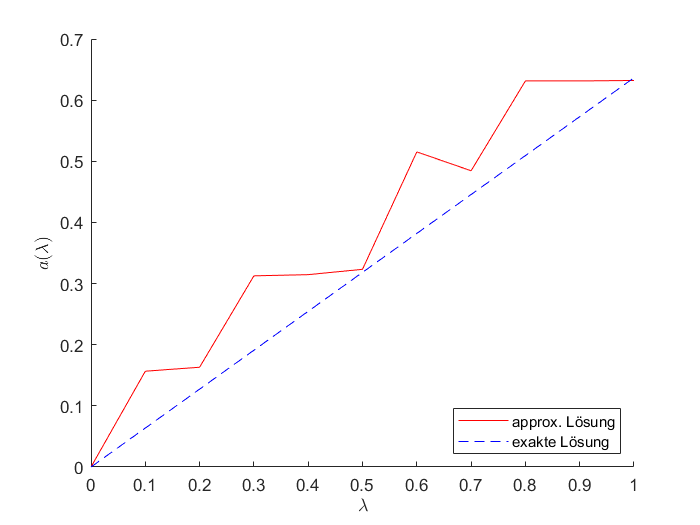
\includegraphics[width=13cm]{epsilon-1.png}
\end{figure}
\newpage

\item[-]$\varepsilon=10^{-2}$: F"ur diese Fehlerschranke gilt L=6.\\[0,3cm]

\begin{tabular}{|c|c|c|c|c|c|c|}
Sampleanzahl &Level 1 & Level 2&Level 3&Level 4&Level 5& Level 6 \\
 \hline
& 16703    &    5906    &    2088     &    739    &     261 &  93\\
\end{tabular}\\[0,3cm]

Es ist zu erkennen, wie viel mehr Samples und Level man ben"otigt um den Fehler um eine Nachkommastelle zu verbessern.
Die Ergebnisse von $a(\lambda)$ sind\\[0,3cm]

\begin{tabular}{|c|c|c|c|c|c|}

$\lambda$ & $0.1$&$0.3$&$0.5$&$0.7$&$1$  \\
 \hline
$a(\lambda)$&  0.0584  &  0.1947 &  0.3204 &   0.4537 &   0.6414\\
\end{tabular}\\

\begin{figure}[h]
\centering
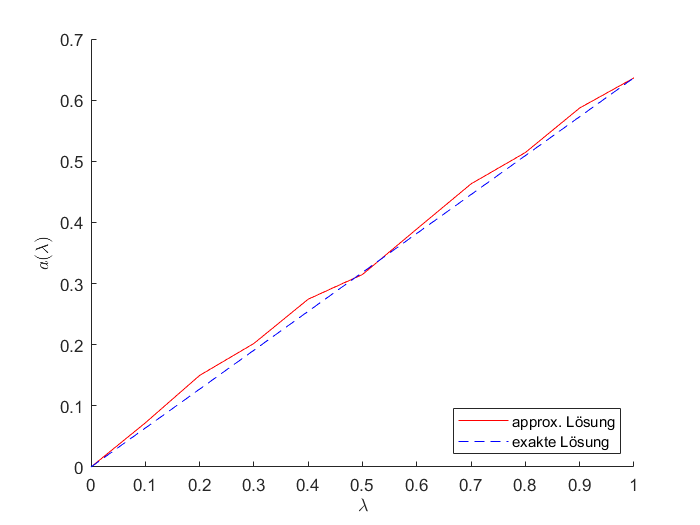
\includegraphics[width=13cm]{epsilon-2.png}
\end{figure}

\newpage

\item[-]$\varepsilon=10^{-3}$:
F"ur diese Fehlerschranke gilt L=9.\\[0,3cm]

\begin{tabular}{|c|c|c|c|c|c|c|}
Sampleanzahl &Level 1 & Level 2&Level 3&Level 4&Level 5& Level 6\\
 \hline
& 4154140   &  1468711  &    519268  &    183589     &  64909 & 22949 \\ 
\end{tabular}\\[0,3cm]

\begin{tabular}{|c|c|c|}
 Level 7 & Level 8 & Level 9\\
 \hline
  8114   &     2869&   1015\\
\end{tabular}\\[0,3cm]
Die Ergebnisse von $a(\lambda)$ sind\\[0,3cm]
\begin{tabular}{|c|c|c|c|c|c|}

$\lambda$ & $0.1$&$0.3$&$0.5$&$0.7$&$1$  \\
 \hline
$a(\lambda)$&  0.0646  &  0.1911  &  0.3183   & 0.4430 &   0.6364\\
\end{tabular}
\begin{figure}[h]
\centering
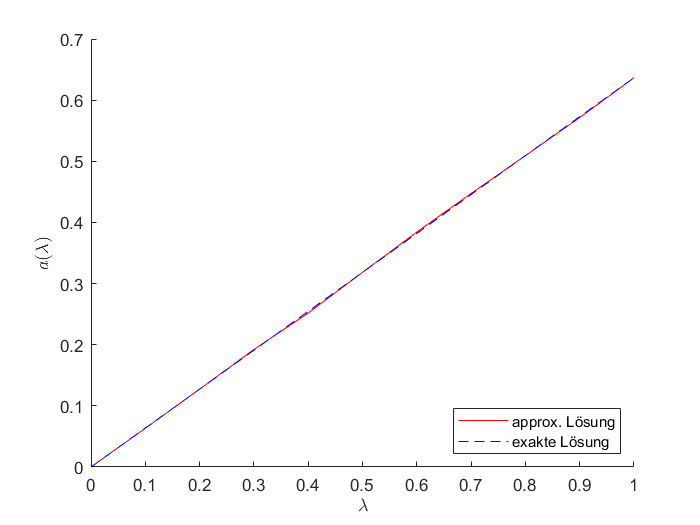
\includegraphics[width=12cm]{epsilon-3.png}
\end{figure}

\item[-]$\varepsilon=10^{-4}$: \\
Ab diesem Fehler war es mir nicht mehr m"oglich mit Matlab die Ergebnisse f"ur $a(\lambda)$ zu bestimmen, da die optimale Sampleanzahl zu gro"s ist.\\
F"ur diese Fehlerschranke gilt L=12.\\[0,3cm]
\begin{tabular}{|c|c|c|c|c|c|c|}
Sampleanzahl &Level 1 & Level 2&Level 3&Level 4&Level 5& Level 6\\
 \hline
$1.0e+09 *$& 3.2314  &  1.1425 &   0.4039   & 0.1428  &  0.0505   & 0.0179  
\end{tabular}\\[0,3cm]
\begin{tabular}{|c|c|c|c|c|c|c|}
 & Level 7 & Level 8 & Level 9& Level 10 &Level 11& Level 12\\
 \hline
$1.0e+09 *$  &  0.0063  &  0.0022 &   0.0008 &  0.0003  &  0.0001 &   0.0000
\end{tabular}\\[0,3cm]

\end{enumerate}

 

 

\newpage
\subsection{Abh"angigkeit der Rechenkosten und der Fehlertoleranz}
Im vorherigen Kapitel haben wir die optimale Anzahl an Samples pro Level bei gegebener Levelanzahl $L\in\mathbb{N}$ und Fehlertoleranz $\varepsilon\in(0,\infty)$  bestimmt. Wegen \eqref{L1} verh"alt sich die untere Schranke f"ur $L\in\mathbb{N}$ wie $(q_1\log(h))^{-1}\log(\varepsilon)$ f"ur $\varepsilon\rightarrow 0$.\\
In diesem Kapitel wollen wir nun die Abh"angigkeit der gesamten Rechenkosten des MLMC-Algorithmus und der Fehlertoleranz untersuchen. Hierf"ur ist es notwendig eine Verbindung von $L$ und $\varepsilon$ herzustellen.\\
Daf"ur sei $\theta\in (0,1)$ und wir definieren
\begin{align}\label{L}
L_\theta:=L_\theta(\varepsilon):=\Big\lceil \frac{\log(\varepsilon)+\log{(\frac{\theta}{C_1}})}{q_1\log(h)}\Big \rceil\in\mathbb{N}.
\end{align}
Dies stellt sicher, dass der Statistische Bias von $\theta\varepsilon$ eingegrenzt wird. Beziehungsweise analog zur Rechnung in \eqref{L1} gilt $C_1h^{q_1L_\theta}\leq \theta\varepsilon$. Also gilt insgesamt:
\begin{align*}
\|a-\mathcal{M}_L^{\text{MLMC}}((n_l)_{l=1}^L)\|_{L^p(\Omega;E)}\leq &\underbrace{C_1 h^{q_1L}}_{\leq \theta\varepsilon}+\underbrace{2C_2 T_p(E)\left(\sum_{l=1}^L \frac{h^{p q_2 l}}{n_l^{p-1}}\right)^{\frac{1}{p}}}_{\leq(1-\theta)\varepsilon}\leq\varepsilon.
\end{align*} Folglich ist
\begin{align*}
\delta_\theta:=\frac{(1-\theta)\varepsilon}{2C_2T_p(E)}\leq \frac{\varepsilon-C_1h^{q_1L_\theta}}{2C_2T_p(E)}=\delta.
\end{align*}
Unser Ziel ist es, das Wachstum von $\text{cost}(\mathcal{M}_{L_\theta}^{\text{MLMC}}((n_l^\theta)_{l=1}^{L_\theta}))$ f"ur $\varepsilon\rightarrow 0$ zu bestimmen. $(n_l^\theta)_{l=1}^{L_\theta}$ beschreibt die Anzahl an Samples in \eqref{n} mit $L_\theta$ und $\delta_\theta$ anstelle von $L$ und $\theta$. Das bedeutet
\begin{align*}
n_l^\theta:=\lceil a_l^\theta \rceil:=\left\lceil \delta_\theta^{-\frac{p}{p-1}}b_lc_l^{-\frac{1}{p}}\left(\sum_{k=1}^{L_\theta} c_k^{\frac{p-1}{p}}b_k\right)^{\frac{1}{p-1}}\right\rceil \in \mathbb{N}, \ \ l=1,...,L_\theta,
\end{align*}
wobei $b_l$ und $c_l$ dieselben wie in \eqref{delta} sind. Wegen $\delta^{-\frac{p}{p-1}}\leq \delta_\theta^{-\frac{p}{p-1}}$ folgt, dass auch $n_l^*\leq n_l^\theta$ f"ur $l=1,...,L_\theta$ gilt. Daher ist $(n_l^\theta)_{l=1}^{L_\theta}$ eine geeignete L"osung f"ur $(6)-(8)$ mit 
\begin{align*}
\text{cost}(\mathcal{M}_{L_\theta}^{\text{MLMC}}((n_l^*)_{l=1}^{L_\theta}))\leq \text{cost}(\mathcal{M}_{L_\theta}^{\text{MLMC}}((n_l^\theta)_{l=1}^{L_\theta})).
\end{align*}
Au"serdem ist mit Voraussetzung \ref{v} eine obere Schranke f"ur die Kosten gegeben. Diese ergibt sich aus
\begin{align}\label{r}
\text{cost}(\mathcal{M}_{L_\theta}^{\text{MLMC}}((n_l^\theta)_{l=1}^{L_\theta}))
\leq& \nonumber \sum_{l=1}^{L_\theta}n_l^\theta C_3h^{-rl}\leq \sum_{l=1}^{L_\theta}(a_l^\theta+1)C_3h^{-rl}\\ \nonumber=&
\underbrace{C_3\sum_{l=1}^{L_\theta}h^{-rl}}_{(*)}+\underbrace{C_3\sum_{l=1}^{L_\theta}a_l^\theta h^{-rl}}_{(**)}
\\=&C_3\frac{h^{-rL_\theta}-1}{1-h^r}+\delta_\theta^{-\frac{p}{p-1}}\left(\sum_{l=1}^{L_\theta}c_l^{\frac{p-1}{p}}b_l\right)^{\frac{p}{p-1}}.
\end{align}
Der Summand $(*)$ liefert
\begin{align*}
C_3\sum_{l=1}^{L_\theta}h^{-rl}=C_3\sum_{l=0}^{L_\theta-1}(h^{-r})^{l+1}=C_3h^{-r} \sum_{l=0}^{L_\theta-1}(h^{-r})^{l}=C_3h^{-r}\frac{(h^{-r})^{L_\theta}-1}{h^{-r}-1}=C_3\frac{h^{-rL_\theta}-1}{1-h^r}
\end{align*}
und f"ur  $(**)$ gilt
\begin{align*}
C_3\sum_{l=1}^{L_\theta}a_l^\theta h^{-rl}=&C_3\sum_{l=1}^{L_\theta}\delta_\theta^{-\frac{p}{p-1}}b_lc_l^{-\frac{1}{p}}\left(\sum_{k=1}^{L_\theta}c_k^{\frac{p-1}{p}}b_k\right)^{\frac{1}{p-1}}\cdot h^{-rl}
\\=&\delta_\theta^{-\frac{p}{p-1}}\sum_{k=1}^{L_\theta}\left(c_k^{\frac{p-1}{p}}b_k\right)^{\frac{1}{p-1}}\sum_{l=1}^{L_\theta}(b_l\underbrace{c_l^{-\frac{1}{p}}\underbrace{C_3h^{-rl}}_{c_l}}_{c_l^{\frac{p-1}{p}}})\\
=&\delta_\theta^{-\frac{p}{p-1}}\left(\sum_{l=1}^{L_\theta}c_l^{\frac{p-1}{p}}b_l\right)^{\frac{1}{p-1}+1}=\delta_\theta^{-\frac{p}{p-1}}\left(\sum_{l=1}^{L_\theta}c_l^{\frac{p-1}{p}}b_l\right)^{\frac{p}{p-1}}.
\end{align*}
Wegen \eqref{L} ist
\begin{align*}
h^{cL_\theta}=\exp(c\log(h)L_\theta)\leq&\exp\left(c\log(h)\left(\frac{\log(\varepsilon)+\log(\frac{\theta}{C_1})}{q_1\log(h)}+1\right)\right)\\
=&\exp(c\log(h))\cdot\exp\left(c\frac{\log(\varepsilon)+\log(\frac{\theta}{C_1})}{q_1}\right)=h^c\cdot\left(\frac{\varepsilon\theta}{C_1}\right)^{\frac{c}{q_1}}
\end{align*}
f"ur jedes $c\in\mathbb{R}$ erf"ullt.
Damit erhalten wir f"ur den ersten Summanden
\begin{align}\label{1}
C_3\frac{h^{-rL_\theta}-1}{1-h^r}\leq C_3\frac{h^{-rL\theta}}{1-h^r}\leq C_3\frac{1}{h^r(1-h^r)}\left(\frac{C_1}{\theta}\right)^{\frac{r}{q_1}}\varepsilon^{-\frac{r}{q_1}}.
\end{align}
Nachdem wir $b_l$ und $c_l$ eingesetzt haben, erhalten wir mit der geometrischen Reihe
\begin{align}\label{cases}
\sum_{l=1}^{L_\theta}c_l^{\frac{p-1}{p}}b_l=C_3^{\frac{p-1}{p}}\sum_{l=1}^{L_\theta}h^{(q_2-\frac{p-1}{p}r)l}=\begin{cases} C_3^{\frac{p-1}{p}}\frac{1-h^{(q_2-\frac{p-1}{p}r)L_\theta}}{h^{-(q_2-\frac{p-1}{p}r)}-1}, \ \ &\text{falls} \ q_2-\frac{p-1}{p}r>0, \\
C_3^{\frac{p-1}{p}}L_\theta, &\text{falls} \ q_2-\frac{p-1}{p}r=0, \\
C_3^{\frac{p-1}{p}}\frac{h^{(q_2-\frac{p-1}{p}r)L_\theta}-1}{1-h^{-(q_2-\frac{p-1}{p}r)}}, \ \ &\text{falls} \ q_2-\frac{p-1}{p}r<0.\\
\end{cases}
\end{align}
Wir untersuchen nun die drei F"alle im Einzelnen.\\
\underline{1.Fall:}\\
Falls  $q_2-\frac{p-1}{p}r>0$ erhalten wir mit \eqref{cases} und $h\in(0,1)$, dass 
\begin{align*}
\sum_{l=1}^{L_\theta}c_l^{\frac{p-1}{p}}b_l\leq C_3^{\frac{p-1}{p}}\frac{1}{h^{-(q_2-\frac{p-1}{p}r)}-1}
\end{align*} gilt.
Also folgt in diesem Fall mit \eqref{r} und \eqref{1}
\begin{align*}
\text{cost}(\mathcal{M}_{L_\theta}^{\text{MLMC}}((n_l^\theta)_{l=1}^{L_\theta}))\leq& \frac{C_3}{h^r(1-h^r)}\left(\frac{C_1}{\theta}\right)^{\frac{r}{q_1}}\varepsilon^{-\frac{r}{q_1}}+C_3\delta_\theta^{-\frac{p}{p-1}}(h^{-(q_2-\frac{p-1}{p}r)}-1)^{-\frac{p}{p-1}}\\
\underset{(*)}{\leq}& \frac{C_3}{h^r(1-h^r)}\left(\frac{C_1}{\theta}\right)^{\frac{r}{q_1}}\varepsilon^{-\frac{r}{q_1}}+C_3\left(\frac{2C_2T_p(E)}{(1-\theta)(h^{-(q_2-\frac{p-1}{p}r)}-1)}\right)^{\frac{p}{p-1}}\varepsilon^{-\frac{p}{p-1}}\\
\leq& C\left(\varepsilon^{-\frac{r}{q_1}}+\varepsilon^{-\frac{p}{p-1}}\right).
\end{align*}
\begin{enumerate}
\item[-]$(*)$ entsteht durch Einsetzen von $\delta_\theta$.
\item[-]C ist eine Konstante, welche von $C_1,C_2,C_3,T_p(E),h,r,q_1,q_2,p$ und $\theta$ abh"angt.
\end{enumerate}
\underline{2. Fall:}\\
Sei nun also $q_2-\frac{p-1}{p}r=0$. Dann folgt
\begin{align*}
\text{cost}(\mathcal{M}_{L_\theta}^{\text{MLMC}}((n_l^\theta)_{l=1}^{L_\theta}))\leq& \frac{C_3}{h^r(1-h^r)}\left(\frac{C_1}{\theta}\right)^{\frac{r}{q_1}}\varepsilon^{-\frac{r}{q_1}}+C_3\delta_\theta^{-\frac{p}{p-1}}L_\theta^{\frac{p}{p-1}}.
\end{align*}
Durch Absch"atzen nach oben von $L_\theta$ und Einsetzen von $\delta_\theta$ erhalten wir
\begin{align*}
C_3\delta_\theta^{-\frac{p}{p-1}}L_\theta^{\frac{p}{p-1}}\leq& C_3\left(\frac{2C_2T_p(E)}{(1-\theta)\varepsilon}\right)^{\frac{p}{p-1}}\left(\frac{\log(\varepsilon)+\log(\frac{\theta}{C_1})}{q_1\log(h)}+1\right)^{\frac{p}{p-1}}\\
\leq& C(1+\log(\varepsilon^{-1})^{\frac{p}{p-1}})\varepsilon^{-\frac{p}{p-1}}.
\end{align*}
Insgesamt existiert dann eine Konstante $C$, welche von $C_1,C_2,C_3,T_p(E),h,r,q_1,q_2,p$ und $\theta$ abh"angt, sodass gilt:
\begin{align*}
\text{cost}(\mathcal{M}_{L_\theta}^{\text{MLMC}}((n_l^\theta)_{l=1}^{L_\theta}))\leq C(\varepsilon^{-\frac{r}{q_1}}+(1+\log(\varepsilon^{-1})^{\frac{p}{p-1}})\varepsilon^{-\frac{p}{p-1}}).
\end{align*}
\underline{3.Fall:}\\
Sei nun $q_2-\frac{p-1}{p}r<0$ dann folgt aus \eqref{1} mit $(q_2-\frac{p-1}{p}r)L_\theta$ anstelle von $-r$
\begin{align*}
\frac{h^{(q_2-\frac{p-1}{p}r)L_\theta}-1}{1-h^{-(q_2-\frac{p-1}{p}r)}}\leq \frac{1}{h^{-(q_2-\frac{p-1}{p}r)}(1-h^{(q_2-\frac{p-1}{p}r)})}\left(\frac{C_1}{\theta}\right)^{-\frac{1}{q_1}(q_2-\frac{p-1}{p}r)}\varepsilon^{\frac{1}{q_1}(q_2-\frac{p-1}{p}r)}.
\end{align*}
Also erhalten wir in diesem Fall
\begin{align*}
\text{cost}(\mathcal{M}_{L_\theta}^{\text{MLMC}}((n_l^\theta)_{l=1}^{L_\theta}))\leq C\left(\varepsilon^{-\frac{r}{q_1}}+\varepsilon^{-\frac{p}{p-1}(1-\frac{1}{q_1}(q_2-\frac{p-1}{p}r))}\right).
\end{align*}
Wir befinden uns mit unseren Konstanten im ersten Fall, da $q_2-\frac{p-1}{p}r=1- \frac{2-1}{2}\cdot 1 = 1- \frac{1}{2}=\frac{1}{2}>0$ ist. Dies bedeutet, dass f"ur unsere Kosten gilt:
\begin{align*}
\text{cost}(\mathcal{M}_{L_\theta}^{\text{MLMC}}((n_l^\theta)_{l=1}^{L_\theta}))\leq C\left(\varepsilon^{-1}+\varepsilon^{-2}\right).
\end{align*}
Wegen
\begin{equation*}
\lim_{\varepsilon\rightarrow 0} \frac{\frac{1}{\varepsilon}}{\frac{1}{\varepsilon^2}}=\lim_{\varepsilon\rightarrow 0} \varepsilon=0
\end{equation*}
dominiert $\varepsilon^{-2}$ den Term $\varepsilon^{-1}$  und
unsere Kosten sind von Ordnung $\mathcal{O}(\varepsilon^{-2})$ . Dies ist besser als die der klassischen Monte-Carlo-Methode mit $\mathcal{O}(\varepsilon^{-3})$.\\[0,2cm]
Es ist wieder die genaue Kenntnis der Konstanten $C_1,C_2,T_p(E),h$ sowieso der Raten $q_1,q_2$ und $r$ vonn"oten. In der Praxis sind diese Variablen nicht alle verf"ugbar. Jedoch gilt trotzdem, dass die Verh"altnisse der $(n_l^*)_{l\in\mathbb{N}}$  nicht von $C_1,C_2$ und $T_p(E)$ abh"angen. Denn es ist
\begin{align*}
\frac{a_l^*}{a_1^*}=h^{(q_2+\frac{r}{p})(l-1)} 
\end{align*} f"ur $l=1,2,...L$.
Die Strategie ist nun den MLMC-Algorithmus mit der Wahl
\begin{align*}
\overline{n_l}:=\lceil \eta_\varepsilon h^{-(q_2+\frac{r}{p})(L-l)} \rceil,
\end{align*}
zu implementieren.
Hierbei ist $\eta_\varepsilon\in (0,\infty)$ ein Parameter, der von der Fehlertoleranz $\varepsilon>0$ abh"angt. Die Gleichung\eqref{n} liefert, dass $\eta_\varepsilon$ sich asymptotisch wie $\varepsilon^{-\frac{p}{p-1}}$ f"ur $\varepsilon\rightarrow0$ verh"alt.
\subsection{Optimale Anzahl von Leveln und Samples bei gegebenen Rechenaufwand}
Im vorherigen Kapitel haben wir uns einen Fehler $\varepsilon>0$ und damit auch die Levelanzahl $L\in\mathbb{N}$ vorgegeben. Davon ausgehend, unter der Bedingung die Kosten minimal zu halten, dann die optimale Sampleanzahl bestimmt.\\
In diesem Kapitel besch"aftigen wir uns damit, unter Vorgabe eines Kostenbudgets $C$ die optimale Levelanzahl sowie die optimale Anzahl an Samples auf jedem dieser Level zu bestimmen, sodass wir aber einen m"oglichst kleinen Fehler haben.\\[0,2cm]

Eine obere Schranke f"ur die Anzahl der Level ist automatisch gegeben.
Angenommen wir nehmen auf jedem Level nur ein Sample, dann gilt:
\begin{align}
\sum_{l=1}^L C_3 h^{-l} \leq C \Leftrightarrow& \sum_{l=1}^L 2^l \leq \underbrace{\frac{C}{C_3}}_{=C'} \underset{geo. Reihe}{\Leftrightarrow} \frac{1-2^{L+1}}{1-2}-1\leq C' 
\Leftrightarrow 1-2^{L+1}+1 \geq -C'\\
 \Leftrightarrow & 2+C' \geq 2^{L+1} \Leftrightarrow \frac{\ln(2+C')}{\ln(2)}-1\geq L 
\end{align}
Nat"urlich wird es nicht vorkommen, dass man nur ein Sample pro Level nimmt. Dies war nur eine rein theoretische Annahme um "uberhaupt eine Schranke f"ur die Levelanzahl zu erhalten. Diese schwache Schranke garantiert jedoch, dass wir nur endlich viele Level testen m"ussen.
Das Ziel ist es nun, einen Algorithmus zu entwickeln, der unser eigentliches Problem l"ost.\\[0,1cm]

Zuerst besch"aftigen wir uns jedoch wieder damit, dass die Levelanzahl $L\in\mathbb{N}$ fest gegeben sei. Wir bestimmen dann die optimale Anzahl an Samples auf jedem dieser Level. Jedoch unter der Bedingung, dass die Kosten unter der vorgegebenen Schranke $C$ liegen.\\
Danach gilt es rauszufinden, welche Levelanzahl optimal ist. Wegen $(18)$, wissen wir unsere maximale Anzahl an theoretisch m"oglichen Leveln. Da wir aber mehr als nur ein Sample auf den verschiedenen Leveln nehmen, wird die tats"achliche Levelanzahl stark darunter liegen. Jedoch werde ich von dieser Schranke ausgehen, um die optimale Levelanzahl zu bestimmen.\\[0,1cm]
D.h. wir haben nun f"ur gegebenes $L,C \in \mathbb{N}$ folgendes Problem zu l"osen:
\begin{align*}
\min_{(n_1,n_2,...,n_L)\in\mathbb{N}^L}& \|a-\mathcal{M}_L^{\text{MLMC}}((n_l)_{l=1}^L)\|_{L^p(\Omega;E)}\\
\text{\small{u.d.N}}& \sum_{l=1}^L n_l \cdot c_l \leq C
\end{align*}
Wir haben eine obere Schranke f"ur $\|a-\mathcal{M}_L^{\text{MLMC}}((n_l)_{l=1}^L)\|_{L^p(\Omega;E)}$ gegeben. 
Wir wollen nun also diese Schranke optimieren.\\
 Mit unseren schon in den vorherigen Kapiteln bestimmten Konstanten ergibt sich die Schranke
\begin{align*}
\frac{2}{\pi\sqrt{3}}\left(\frac{1}{2}\right)^L+\frac{2}{\pi}\left(\sum_{l=1}^L\left(\frac{1}{4}\right)^l\cdot\frac{1}{n_l}\right)^{\frac{1}{2}}.
\end{align*}
Da der erste Summand nicht von $n_l$ abh"angt, kann man diesen f"ur die Minimierung vernachl"assigen. Genauso den Faktor $\frac{2}{\pi}$ im zweiten Summanden. Aufgrund der Monotonie der Wurzelfunktion reicht es also $\sum_{l=1}^L\frac{1}{4}^l\cdot\frac{1}{n_l}$ zu minimieren. Wir erhalten also mit der zu Anfang des Kapitel 5 bestimmten Schranke f"ur die Kosten folgendes vereinfachte Optimierungsproblem
\begin{align*}
\min_{(n_1,n_2,...,n_L)\in\mathbb{N}^L}&\sum_{l=1}^L(\frac{1}{4})^l\cdot\frac{1}{n_l}\\
\text{\small{u.d.N}}& \sum_{l=1}^L n_l \frac{5}{2}2^l\leq C\\
\Leftrightarrow& \sum_{l=1}^L n_l 2^l\leq \underbrace{C \cdot \frac{2}{5}}_{C'}.
\end{align*}
Wir geben uns also immer die Konstante $C':=C$ vor.\\[0,2cm]

\textbf{\underline{Bemerkung:}}\\
Wenn man die zu minimierende Funktion genauer betrachtet, ist leicht zu erkennen, dass wir die meisten Samples auf den niedrigen Leveln und vor allem auf Level 1 nehmen m"ochten. Da der Faktor $\frac{1}{4^l}$ mit gr"o"ser werdendem $l$ immer geringer wird, ist es f"ur unseren Fehler $\varepsilon$ am schlechtesten die $n_l$ f"ur niedrige $l$ zu verringern. Dies w"urde das schnellste Wachstum des Funktionswertes  bedeuten.\\[0,2cm]
Nun werde ich meine zwei Vorgehensweisen zur Bestimmung eines Optimums vorstellen. Dabei habe ich immer die Tatsache aus der Bemerkung ber"ucksichtigt.



\newpage
\subsubsection{Die Lagrange-Multiplikator-Methode}
Unter Vernachl"assigung der Ganzzahligkeitsbedingung an die $n_l$ kann dieses Problem durch geschickte Substitution mit Hilfe der Lagrange-Multiplikator-Methode gel"ost werden.
Wir substituieren $4^l\cdot n_l= y_l$ und suchen das Minimum der Funktion $\sum_{l=1}^L \frac{1}{y_l}$ unter der neuen  Nebenbedingung  $\sum_{l=1}^L \left(\frac{1}{2}\right)^l \cdot y_l \leq C$. Da wir die Ganzzahligkeit erstmal vernachl"assigen, wissen wir, dass unsere Nebenbedingung zur Gleichung wird.\\
Wir erhalten also folgende Lagrange-Funktion mit zugeh"origem Gradienten:
\begin{align*}
L(y,\lambda)=&\sum_{l=1}^L \frac{1}{y_l}+\lambda\cdot \left(\sum_{l=1}^L\left(\frac{1}{2}\right)^ly_l-C \right)\\
\nabla L(y,\lambda)=&\begin{pmatrix}
-\frac{1}{y_1^2}+\lambda\cdot \left(\frac{1}{2}\right)^1\\
\vdots\\
-\frac{1}{y_L^2}+\lambda\cdot \left(\frac{1}{2}\right)^L\\
\sum_{l=1}^L \left(\frac{1}{2}\right)^ly_l-C
\end{pmatrix}\overset{!}{=}0
\end{align*} mit $y=(y_1,...,y_L)$.
Wir erhalten f"ur die $l$-te Komponente
\begin{align*}
\lambda\cdot \left(\frac{1}{2}\right)^l=\frac{1}{y_l^2} \Leftrightarrow y_l^2=\frac{1}{\lambda}\cdot 2^l \Leftrightarrow y_l=\frac{\sqrt{2^l}}{\sqrt{\lambda}},
\end{align*}
sowie
\begin{align*}
\sum_{l=1}^L   \frac{\sqrt{2^l}}{\sqrt{\lambda}} \cdot\left(\frac{1}{2}\right)^l=C\Leftrightarrow \frac{1}{C}\sum_{l=1}^L (\sqrt{2})^{-l}=\sqrt{\lambda}.
\end{align*}
Das bedeutet wir erhalten insgesamt $y_l=\frac{\sqrt{2^l}\cdot C}{\sum_{l=1}^L(\sqrt{2})^{-l}}$ und durch Resubstitution folgt f"ur die optimale Sampleanzahl
\begin{align*}
n_l=\frac{\sqrt{2^l}\cdot C}{4^l\sum_{l=1}^L(\sqrt{2})^{-l}}.
\end{align*}
Diese ist jedoch noch nicht ganzzahlig. Um dieses Problem zu umgehen, kann man wie im vorherigen Kapitel die untere Gau"sklammer auf diese $n_l$ anwenden. Dies wird also nahe am Optimum liegen. Durch das Abrunden der einzelnen Zahlen werden jedoch Kosten frei, da durch die $n_l$ mit Lagrange die Summe der einzelnen Samplekosten genau C ergeben haben.\\
Die Idee ist nun, die Samples auf Level $1$ ( mit den niedrigsten Kosten und gr"o"sten Vorfaktor $\frac{1}{4}$) um $1$ zu erh"ohen, solange  wir dadurch immer noch unter unserer Kostenschranke $C$ bleiben. Dies verringert den Fehler $\varepsilon$ sicher.\\
Durch das Abrunden der einzelnen Sampleanzahlen kann es jedoch vorkommen, dass wir auf Null abrunden. Dies geschieht bei einem zu geringen Kostenbudget und daf"ur zu hoher gew"unschter Levelanzahl. In diesem Fall ignorieren wir die auf Null gerundeten Level
und geben den Fehler \textit{"Levelanzahl zu hoch f"ur diese Kosten. Levelanzahl senken oder Kosten erh"ohen."} aus.\\[0,2cm]
\textbf{Beispiele:}
\begin{enumerate}
\item[a)] Ausgabe f"ur $C=100$:
\begin{enumerate}
\item[-]1 Level: $n=50$; $\varepsilon=0.2288$
\item[-]2 Level: $n=(30,10)$ ; $\varepsilon=0.1688$
\item[-]3 Level: $n=(26,8,2)$;$\varepsilon=0.1471$
\item[-]4 Level: 
 $n=( 30,6,2);\varepsilon= 0.1497$.\\
F"ur diese Levelanzahl sind die Kosten zu hoch und obige Fehlermeldung wird ausgegeben. 
D.h. bei diesen Kosten sind $4$ Level nicht mehr sinnvoll und es wurde nach 3 Leveln abgeschnitten.
\end{enumerate}
\item[b)] Ausgabe f"ur $C=1000$:  Hier ist schon eine deutliche Verbesserung des Fehlers im Vergleich zu a) zu erkennen.

\item[-]2 Level: $n=(294,103); \varepsilon= 0.1162$
\item[-]4 Level: $n=(202,69,24, 8);\varepsilon= 0.0594$
\item[-]5 Level: $n=(200,62,22,7,2);\varepsilon=0.0518$
\item[-]6 Level: $n=(214,59,20,7,2);\varepsilon=0.0520$\\
F"ur diese Levelanzahl sind die Kosten zu hoch und obige Fehlermeldung wird ausgegeben. 
\item[c)] Ausgabe f"ur $C=10000$:
\item[-]4 Level: $n=(1956,690,24,86);\varepsilon=0.0345$
\item[-]6 Level: $n=(1694,591,209,73,26,9);\varepsilon= 0.0192$
\item[-]8 Level: $n=(1604,552,195,69,24,8,3,1);\varepsilon=0.0158$\\
Ab Level 9 ist das Kostenbudget zu niedrig.
\end{enumerate}
Bisher haben wir also unter Vorgabe des Kostenbudgets sowie der gew"unschten Levelanzahl die optimale Verteilung der Samples bestimmt, sofern dies von der Kapazit"at m"oglich ist.
Nun gilt es die \textbf{optimale Levelanzahl} herauszufinden.\\
Hierbei bin ich folgenderma"sen vorgegangen:\\
Es ist klar, dass bei gleichbleibendem Kostenbudget $C$ aber einer h"oheren Levelanzahl weniger Samples auf den bisherigen Level genommen werden m"ussen. Dies ist notwendig um sich die Samples auf dem neuen zus"atzlichen Level leisten zu k"onnen. Eine Verringerung der Sampleanzahlen bedeutet aber eine Vergr"o"serung unseres zweiten Summanden in der Schranke f"ur $\varepsilon$. \\
Zu Erinnerung: Die Schranke, welche wir minimieren wollen war
\begin{align*}
\underbrace{\frac{2}{\pi\sqrt{3}}\left(\frac{1}{2}\right)^L}_{(1)}+ \underbrace{\sum_{l=1}^L\left(\frac{1}{4}\right)^l\cdot\frac{1}{n_l}}_{(2)}.
\end{align*}
Eine Erh"ohung der Levelanzahl l"asst also $(2)$ wachsen. Jedoch wird $(1)$ f"ur ein gr"o"ser werdendes $L$ schnell klein. Die Frage ist nun, wie weit wir $L$ erh"ohen k"onnen, sodass die Verringerung in $(1)$ die Erh"ohung in $(2)$ "ubertrifft.
Deshalb gehe ich von der in $(18)$ bestimmten Anzahl an maximalen Leveln aus und wende den auf der n"achsten Seite beschriebenen Algorithmus an.
Dieser wird die in $(18)$ beschriebene Schranke sinnvoll reduzieren und anschlie"send alle Level bis zu dieser  neuen Schranke durchgehen. Die Ergebnisse f"ur $\varepsilon$ werden dann verglichen  und die Levelanzahl mit dem kleinsten $\varepsilon$ ausgew"ahlt.\newpage 
Das Vorgehen zum bestimmen der optimalen Levelanzahl sieht also folgenderma"sen aus:\\

\begin{algorithm}[H]
$\text{maxL}= \lfloor\frac{\log( cost + 2)}{\log(2)} -1\rfloor;$\\
temp(l) =$\left\lfloor \frac{\sqrt{2^l}\cdot C}{4^l\sum_{l=1}^{maxL}(\sqrt{2})^{-l}}\right\rfloor$ \text{f"ur $l=1,..,maxL$}
\text{\%Abgerundete optimale Sampleanzahlen bei einem Kostenbudget C}\\
\For{i=1 \textbf{to} maxL}{ 
    \If {temp(i) == 0}{
        maxL = i-1; }}
        \For{L=1 \textbf{to} maxL}{bestimme optimale Sampleanzahl und $\varepsilon$ mit Lagrange }
Suche das $L$ mit minimalen $\varepsilon$.\\[0,5cm]


\caption{Algorithmus f"ur optimale Sample-und Levelanzahl mit der Lagrange-Methode}
\end{algorithm}\vspace{0,3cm}
Nachfolgend eine Tabelle mit den Ergebnissen:\\
\begin{center}
\begin{tabular}{|c|c|c|}
Kostenbudgets & opt. Levelanzahl & Fehler $\varepsilon$ \\
 \hline
10 & 1 & 0.3261 \\
\hline
100& 3 & 0.1471 \\
\hline
1000& 5 &  0.0518 \\
\hline
10 000& 8 & 0.0158 \\
\hline
100 000& 10 & 0.0051 \\
\hline
1 000 000& 12 &  0.0016 \\
\hline
5 000 000& 13 & 7.2485e-04
 \\
\end{tabular}
\end{center}\vspace{0,2cm}
Wie zu erwarten sinkt der Fehler mit wachsendem Kostenbudget, da dadurch eine h"ohere Levelanzahl m"oglich ist. Eine h"ohere Levelanzahl bedeutet eine feinere Diskretisierung und das Ergebnis wird genauer.\\
Vergleichen wir die optimale Levelanzahl mit den Ergebnissen aus dem Beispiel davor, ist zu erkennen, dass die gr"o"stm"ogliche Levelanzahl bei dem vorgegebenen Kostenbudgets den kleinsten Fehler liefert.  

Die zugeh"origen Sampleverteilungen zur obiger Tabelle sind:
\begin{center}
\begin{tabular}{|c|c|}
Kostenbudgets & Sampleverteilung \\
 \hline
10 & n=5 \\
\hline
100& n=(26,8,2) \\
\hline
1000& n=(200,62,22,7,2)\\
\hline
10 000& n=(1604,552,195,69,24,8,3,1)\\
\hline
100 000& n=(15564,5344,1889,668,236,83,29,10,3,1)\\
\hline
1 000 000& n=(151252,52598,18596,6574,2324,821,290,102,36,12,4,1)\\
\hline
5 000 000& n=(747166,261775,92551,32721,11568,4090,1446,511,180)
 \\
\end{tabular}
\end{center}\vspace{0,3cm}
Vergleichen wir nun diese Ergebnisse mit denen aus Kapitel 5.1.
% Um den Unterschied der Probleme nochmal zu wiederholen,
In Kapitel 5.1 haben wir uns die Fehlerschranke sowie die Levelanzahl vorgegeben
und wollten den Fehler $\varepsilon$ unter m"oglichst geringen Kosten erreichen. In unserem aktuellen Problem wollen wir den Fehler minimieren und haben die Kosten vorgegeben.\\
%F"ur einen Fehler von $10^{-1}$ lieferte 5.1 als Ergebnis: \\
Der Abschnitt 5.1 liefert f"ur $\varepsilon = 10^{-1}$ und $L=2$
\begin{align*}
n_L = (2629,930)
\end{align*}
als Ergebnis. Dies ergibt also Kosten von 
\begin{align*}
2629 \cdot 2+ 930 \cdot 4= 8974.
\end{align*}
Die Lagrange-Methode liefert mir bei Vorgabe dieser Kosten und der Vorgabe von 2 Leveln das Ergebnis: 
\begin{align*}
n_L=(2629,929)
\end{align*}
Es ist also zu erkennen, dass die optimale Sampleanzahlen fast die gleichen sind. Dies ist jedoch bei gleicher Vorgabe der Levelanzahl auch zu erwarten. Bestimmen wir jedoch die optimale Levelanzahl und den optimalen Fehler bei diesen Kosten liefert mein Algorithmus das Ergebnis:
\begin{align*}
L=7; \
n=[1541,509,180,63,22,7,2]; \ 
\varepsilon=0,0177
\end{align*}
Es ist also durch eine Erh"ohung der Levelanzahl und anderer Verteilung der Samples ein deutlich besseres Ergebnis bei selben Kosten m"oglich.\\
Mit Kosten von $25 000$ liefert die Lagrange-Methode ein optimales $L=8$ mit einem Fehler von $10^{-2}$.\\
Das Vorgehen aus 5.1 liefert f"ur diese Fehlerschranke mit $L=6$ die Kosten
\begin{align*}
16703\cdot 2+ 5906 \cdot 4+ 2088 \cdot 8+ 739 \cdot 16 + 261 \cdot 32 + 93 \cdot 64 =99862
\end{align*}
Wir sehen bereits, dass der selbe Fehler durch knapp ein Viertel der Kosten erreicht werden kann.
Geben wir jedoch auch der Lagrange-Methode die Levelanzahl $L=6$ vor, erhalten wir den Samplevektor
\begin{align*}
n=[16733,5909, 2089,738,261,92]
\end{align*}
Also wieder das fast gleiche Ergebnis wie aus 5.1.\\
Das Problem bei der Methode aus 5.1 ist, dass wir die Levelanzahl nicht optimiert haben. 
Aus \eqref{L1} geht nur hervor, dass wir die Levelanzahl gr"o"ser als 
\begin{align*}
\frac{\log(\varepsilon)-\log(\frac{1}{\pi\sqrt{3}})}{\log(\frac{1}{2})}
\end{align*} w"ahlen m"ussen. Hier kann es bessere M"oglichkeiten als nur das Aufrunden geben. Das hei"st durch die flexible Levelwahl ist ein viel besseres Ergebnis unter geringeren Kosten m"oglich.
 

\subsubsection{Rucksack-Problem (Greedy-Algorithmus)}
Nun betrachten wir unsere Problemstellung als ein Rucksack-Problem (Knapsack-Problem). Das Volumen des Rucksacks entspricht unserem Kostenbudget. Unser Ziel ist es nun, diesen Rucksack m"oglichst sinnvoll und mit dem f"ur uns besten Nutzen zu packen. In unserem Fall entspricht dies einem m"oglichst kleinen Fehler. Wir haben zum Packen unseres Rucksacks unterschiedliche G"uter mit entsprechendem Gewicht zur Verf"ugung. Bei uns sind diese G"uter die Samples auf den unterschiedlichen Level mit den Kosten $2^l$.
Eine M"oglichkeit solche Probleme zu l"osen sind Greedy-Algorithmen.
Zuerst gilt zu kl"aren, was unter einem Greedy-Algorithmus zu verstehen ist. Hierbei orientiere ich mich an \cite{Greedy}.\\
Greedy-Algorithmen bilden eine spezielle Klasse von Optimierungsalgorithmen. Sie zeichnen sich dadurch aus, dass sie schrittweise den Folgezustand ausw"ahlen, der zum Zeitpunkt der Wahl den gr"o"sten Gewinn bzw. das beste Ergebnis (berechnet durch eine Bewertungsfunktion) verspricht. Greedy-Algorithmen sind oft schnell, l"osen viele Probleme aber nicht optimal.\\[0,1cm]

Ein gieriger Algorithmus m"ochte in jedem Teilschritt so viel wie m"oglich im Hinblick auf die Vorgabe erreichen. Eine Anwendung eines solchen Greedy-Algorithmus im t"aglichen Leben ist beispielsweise die Herausgabe von Wechselgeld.\\[0,1cm]

Das Ziel ist es, eine bestimmte Geldsumme in m"oglichst wenigen Schritten herauszugeben.
Vorgehen nach Greedy: Man nimmt die gr"o"ste M"unze unter dem Zielwert und zieht sie von diesem ab. Man macht dies solange, bis der Zielwert gleich Null ist. Will man beispielsweise 79 Cent zur"uckgeben, f"angt der Algorithmus sofort mit dem h"ochsten M"unzwert an und macht weiter, bis er den niedrigsten M"unzwert erreicht hat (falls das n"otig ist): 
\begin{align*}
79=50 + 20 + 5 + 2 +2
\end{align*}
In diesem Fall klappt das perfekt. Greedy-Algorithmen berechnen jeweils ein  \glqq lokales Optimum\grqq{ } in jedem Schritt und k"onnen daher eventuell ein \glqq globales Optimum\grqq{ } verpassen.\\ Hierf"ur ein Beispiel:\\
Der Zielwert sei $15$. Es stehen M"unzen mit den Werten 1, 5 und 11 zur Verf"ugung.\\
Die optimale L"osung ist $15=5+5+5$. Greedy liefert uns jedoch $15=11+1+1+1+1$.\\[0,5cm]
Mein Ziel ist es nun, durch solch eine Vorgehenswei"se meine optimalen Sampleanzahlen zu bestimmen. In unserem Fall sind wir \glqq gierig\grqq{ } auf Level $1$, da diese Samples, wie schon beschrieben, den gr"o"sten Faktor in der Fehlerfunktion haben.\\
Haben wir zum Beispiel ein Kostenbudget von $C=100$ gegeben, w"urde uns Greedy $50$ Samples auf Level 1 mit Kosten 2 liefern.
Gebe ich vor $2$ Level zu wollen, w"are das Ergebnis $100=48 \cdot 2+ 1\cdot 4$. Dass dieses Ergebnis nicht optimal, ist klar.\\
Mein Ziel ist es nun, durch Umverteilen der Samples das Optimum zu finden.
Dies bedeutet, ich gebe wie auch bei der Lagrange-Methode zuerst eine feste Levelanzahl vor. Der Ausgangspunkt nach Greedy wird immer sein, so viele Samples auf Level 1 wie m"oglich zu nehmen und auf den anderen jeweils nur einen. Solange sich das Ergebnis dadurch verbessert und die Sample Anzahl nicht 0 oder negativ wird, verteile ich Samples von Level 1 auf Level 2. Wird das Ergebnis schlechter, beginne ich mit dem Umverteilen von Level 2 auf Level 3 usw. \\
Da sich die Kosten zweier aufeinanderfolgender Level um den Faktor 2 unterscheiden, folgt, dass die Erh"ohung um ein Sample auf Level $l$ eine Verringerung der Sampleanzahl um zwei bei Level $l-1$ ben"otigt.
Au"serdem brechen wir ab bzw. geben eine Warnung aus, falls wir auf mehreren Leveln hintereinander nur 1 Sample nehmen w"urden. Dies passiert, falls wir nicht mehr weiter umverteilen k"onnen. Da unsere Samples eine monoton fallende Folge bilden m"ussen, macht solch eine Verteilung keinen Sinn. \newpage
Ein Beispiel: Kostenbudget von $C=100$ und eine gew"unschte Levelanzahl von $5$. \\
Das Ergebnis ist:\\
\begin{center}
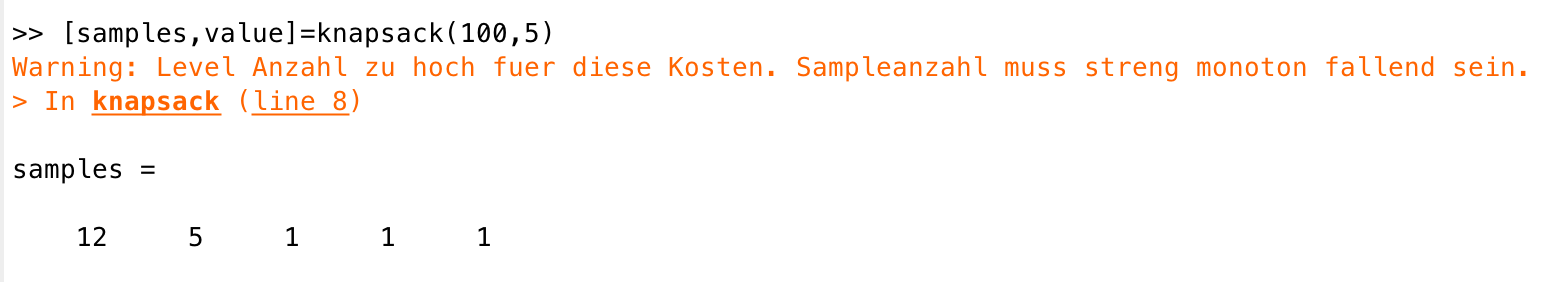
\includegraphics[width=15cm]{Knapsack5.png}
\end{center}
Es konnte also von Level 2 auf Level 3 nicht mehr umverteilt werden, ohne das Ergebnis zu verschlechtern. Deshalb bleiben dann auch alle anderen Samplezahlen unver"andert. Bei einem Kostenbudgets von $100$ ist es also nicht mehr sinnvoll $5$ Level zu fordern. Im Vergleich hierzu das Ergebnis bei nur $4$ Leveln:\\
\begin{center}
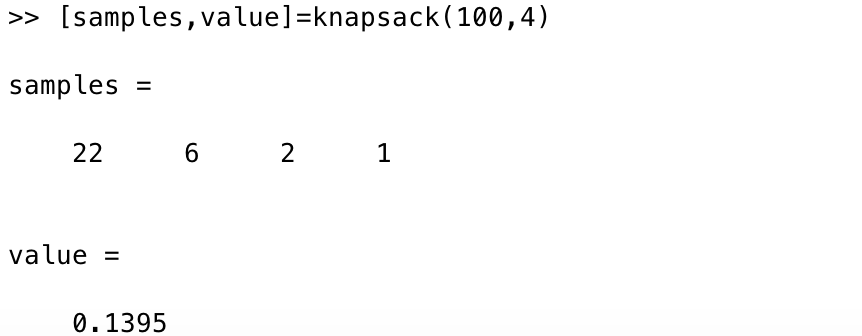
\includegraphics[width=10cm]{Knapsack4.png}
\end{center}
Um nachfolgenden Algorithmus besser zu verstehen, noch ein paar Vor"uberlegungen:\\
Unsere Ausgangssituation ist es, auf jedem Level ab 2 bis L nur ein Sample zu nehmen und so viele wie m"oglich auf Level 1. Hier muss nat"urlich erst "uberpr"uft werden, ob dies "uberhaupt m"oglich ist. Das Kostenbudget k"onnte f"ur die gew"unsche Levelanzahl zu niedrig sein. Ist dies jedoch m"oglich, k"onnen die Kosten der Samples auf Level 2 bis L durch eine geometrische Summe beschrieben werden. N"amlich $\sum_{l=2}^L 1\cdot 2^l = -(1-2^{L+1})-3$. D.h die Sampleanzahl auf Level 1 ist die abgerundete und halbierte (da die Kosten auf Level 1 zwei betragen) Differenz aus dem Kostenbudget und dem Wert der geometrischen Summe.
Auf der n"achsten Seite ist der Algorithmus beschrieben. L ist hierbei die Levelanzahl und cost das vorgegebene Kostenbudget.\\

\begin{algorithm}[H]
\textbf{Knapsack}(cost,L)=\\
samples=(1,...,1) mit L"ange L\\
\eIf{geosum- cost$\geq 2$}{
samples(1)=$\lfloor\frac{(\text{cost-geosum})}{2}\rfloor$\\
value= Fehler, den man mit den samples erh"alt.
}
{Fehler: Levelanzahl f"ur gegebenes Kostenbudget zu hoch!}

\For{l=2 \textbf{to} L}{ 
    \If {samples(l-1)$\leq 2$}{
    \If{(samples(l)=1 und samples(l-1)=1) oder l<L}
    {Breche ab. Levelanzahl zu hoch, da keine monton fallende Folge.}}
 }
\While{1}{
tempsamples=samples\\
tempsamples(l-1)=tempsamples(l-1)-2\\
tempsamples(l)=tempsamples(l)+1\\
tempvalue= Fehler unter tempsamples\\
\eIf{tempvalue >value}{
Abbruch, da Ergebnis schlechter wird.
}
{value=tempvalue\\
samples=tempsamples}
}

\caption{Algorithmus f"ur optimale Sampleanzahl mit der Umverteil-Methode}
\end{algorithm}\vspace{0,3cm}
Um die optimale Levelanzahl zu bestimmen gehen wir analog zu Lagrange vor. Das hei"st wir durchlaufen die einzelnen Level und w"ahlen das mit dem kleinsten $\varepsilon$.\\
Nachfolgend eine Tabelle mit den Ergebnissen:\\
\begin{center}
\begin{tabular}{|c|c|c|}
Kostenbudgets & opt. Levelanzahl & Fehler $\varepsilon$ \\
 \hline
10 & 1 & 0.3261 \\
\hline
100& 4 & 0.1395 \\
\hline
1000& 5 &  0.0562 \\
\hline
10 000& 7 & 0.0206 \\
\hline
100 000& 8 & 0.0082 \\
\hline
1 000 000& 10 &   0.0029 \\
\hline
5 000 000& 11 & 0.0015
 \\
\end{tabular}
\end{center}
Auch hier ist wie bei Lagrange deutlich zu erkennen, dass ein h"oheres Kostenbudget  eine Verbesserung des Fehlers mit sich bringt. 
Die zugeh"origen Sampleverteilungen zur Tabelle sind:
\begin{center}
\begin{tabular}{|c|c|}
Kostenbudgets & Sampleverteilung \\
 \hline
10 & n=5 \\
\hline
100& n=(22, 6 ,2 ,1) \\
\hline
1000& n=(276,58,13,5,1) \\
\hline
10 000& n=(2856,592,124,26,6,3,1) \\
\hline
100 000& n=(29142,6037,1252,260,56,13,4,1) \\
\hline
1 000 000&  n=(292296,60538,12539,2597,539,113,24,7,2,1) \\
\hline
5 000 000& n=(1463266, 303055,62766,13001,2694,558,118 ,25,7,2,1)
 \\
\end{tabular}
\end{center}\vspace{0,3cm}
Wir vergleichen auch diese Methode mit der aus Kapitel 5.1. Wir hatten schon bei Lagrange erw"ahnt, dass Kapitel 5.1 f"ur einen Fehler von $10^{-1}$ 2 Level mit 2629 Samples auf Level 1 und 930 Samples auf Level 2 lieferte. Die Kosten waren 8974.
Unsere Umverteil-Methode liefert f"ur dieses Kostenbudget zwei Level  mit 2629 und 929 Samples. Das bedeutet, dass es hier wie auch schon bei Lagrange  keinen wirklichen Unterschied gibt. Geben wir die Kosten sowie die Levelanzahl vor, erhalten wir wie zu erwarten die selben Ergebnisse wie in Kapitel 5.1. Lassen wir die Levelanzahl jedoch variabel, erhalten wir als Optimum bei diesen Kosten sieben Level und einen Fehler von $0.0215$. 

\subsubsection{Vergleich der beiden Vorgehensweisen}
Wir haben nun zwei sehr unterschiedliche Vorgehensweisen zur Bestimmung der optimalen Sampleanzahlen f"ur den bestm"oglichen Fehler kennengelernt. Bei der Bestimmung der optimalen Levelanzahl sind wir bei beiden Methoden jedoch gleich vorgegangen.\\[0,2cm]
Nun betrachten wir die Unterschiede.\\
W"ahrend wir bei der Lagrange-Methode erstmal die Notwendigkeit der Ganzzahligkeit des Optimums vernachl"assigen und das Problem ausgehend von der analytischen L"osung berechnen, bauen wir bei der zweiten Variante unsere L"osung durch gieriges Vorgehen nach und nach auf. Dies macht nat"urlich gro"se Unterschiede in der Laufzeit.
Bei der Lagrange-Methode berechne ich direkt den Vektor mit dem analytischen Optimum. Danach passiert au"ser Abrunden und Auff"ullen des ersten Levels nichts mehr. Dies ist also eine sehr schnelle Vorgehensweise.\\
Bei der zweiten Methode hingegen gibt es wie im Algorithmus zu erkennen viele Schleifen. Bei einen hohen Kostenbudgets kann dies l"anger dauern. Bez"uglich der Laufzeit ist also die Lagrange-Methode besser.\\[0,2cm]
Vergleichen wir nun die Ergebnisse der beiden Methoden:
\begin{center}
\textbf{Ergebnisse von Lagrange}\\[0,1cm]
\begin{tabular}{|c|c|c|}
Kostenbudgets & opt. Levelanzahl & Fehler $\varepsilon$ \\
 \hline
10 & 1 & 0.3261 \\
\hline
100& 3 & 0.1471 \\
\hline
1000& 5 &  0.0518 \\
\hline
10 000& 8 & 0.0158 \\
\hline
100 000& 10 & 0.0051 \\
\hline
1 000 000& 12 &  0.0016 \\
\hline
5 000 000& 13 & 7.2485e-04
 \\
\end{tabular}\\[0,5cm]
\textbf{Ergebnisse nach Umverteilen}\\[0,1cm]
\begin{tabular}{|c|c|c|}
Kostenbudgets & opt. Levelanzahl & Fehler $\varepsilon$ \\
 \hline
10 & 1 & 0.3261 \\
\hline
100& 4 & 0.1395 \\
\hline
1000& 5 &  0.0562 \\
\hline
10 000& 7 & 0.0206 \\
\hline
100 000& 8 & 0.0082 \\
\hline
1 000 000& 10 &   0.0029 \\
\hline
5 000 000& 11 & 0.0015
 \\
\end{tabular}
\end{center}\vspace{0,2cm}
Es ist zu erkennen, dass bei einem niedrigen Kostenbudgets bis zu 10 000 es keine starken Abweichungen der Ergebnisse gibt.
Bei h"oheren Kosten jedoch ist deutlich zu erkennen, wie viel bessere Ergebnisse die Lagrange-Methode liefert. Dies liegt daran, dass wir von der analytischen optimalen L"osung ausgehen. Diese ist zwar nicht ganzzahlig, jedoch bewegen wir uns nur sehr wenig von ihr weg.\\
Die zweite Methode muss es durch das Umverteilen erstmal schaffen, nahe an die eigentlich optimale L"osung heranzukommen. Durch das strenge Vorgehen der Verteilung von links nach rechts kann es sein, dass wir andere M"oglichkeiten von Sampleverteilungen verpassen, welche vielleicht doch ein besseres Ergebnis liefern w"urden. Dies ist eine klare Schw"ache von Greedy-Algorithmen.\\
\\[0,2cm]
Zur graphischen Veranschaulichung noch ein Plot der Ergebnisse:
\begin{center}
\includegraphics[width=14cm]{Vergleich.png}
\end{center}
Der Fehler, den wir durch die Umverteilmethode erhalten, ist bis auf ein paar wenige Ausnahmen schlechter. Dies gilt vor allem ab einem hohen Kostenbudget.\\
Zusammenfassend ist also klar zu erkennen, dass die erste Vorgehensweise besser ist. Sie liefert sowohl bessere Ergebnisse und ist deutlich schneller.
Die Laufzeit der Umverteilungsmethode w"urde sich jedoch noch verbessern lassen, indem man mehr als ein Sample pro Iteration umschichtet.
Dies l"asst sich beispielsweise durch absteigende Zehnerpotenzen realisieren. Um dieses Vorgehen zu skizzieren betrachten 
wir mit 
\begin{align*}
2 \cdot 10^n +4 \cdot 1 + ... + 2^L \cdot 1 \leq C
\end{align*}
eine m"ogliche Ausgangssituation der Umverteilungsmethode.
Wir verteilen nun solange $10^{n-1}$ Sampels von Level 1 zu Level 2, bis die Nebenbedingung verletzt wird.
Dann nehmen wir einen Verteilvorgang zur"uck und verteilen mit einer Zehnerpotenz weniger.
Das Ergebnis von diesem Vorgehen ist identisch zu der Umverteilung von genau einem Sample pro Iteration.
Durch die Zehnerpotenzschritte wird die Anzahl an insgesamt durchgef"uhrten Iterationen jedoch deutlich gesenkt und die Laufzeit somit reduziert.


\newpage 
\thispagestyle{empty}
\quad  
\newpage
\nocite{*}
\bibliographystyle{abbrv}
\bibliography{Literatur}
\newpage 
\thispagestyle{empty}
\quad  
\newpage
\thispagestyle{empty}
\begin{center}\Large{\textbf{Eigenst"andigkeitserkl"arung}} \end{center}\vspace{2cm}
Hiermit versichere ich, dass ich die vorliegende Masterarbeit selbst"andig verfasst habe.
Ich versichere, dass ich keine anderen als die angegebenen Quellen benutzt habe und  die eingereichte Arbeit weder vollst"andig noch in wesentlichen Teilen Gegenstand eines anderen Pr"ufungsverfahren gewesen ist.\\[2cm]
(Unterschrift)
\end{document}